%===================================================================================================
% PREAMBLE
%===================================================================================================
\documentclass[10pt, handout]{beamer}

\usepackage[utf8]{inputenc}
\usepackage[english]{babel}
\usepackage{lipsum}
\usepackage{tabularx}
\usepackage{caption}
\usepackage{booktabs}
\usepackage{graphicx} 

\usetheme{Dresden}

%===================================================================================================
% CONTENT
%===================================================================================================
\begin{document}

\title{Natural Image Denoise and Deblur}
\author{
Vlad-Ștefan Moreanu \and 
Cosmin Eusebiu Patrașcu
}
\date{Iunie 2026}

\maketitle

%===================================================================================================
% TOC
%===================================================================================================
\begin{frame}{Table of Contents}
    \tableofcontents
\end{frame}

%===================================================================================================
% INTRODUCTION
%===================================================================================================
\section{Introduction}
\begin{frame}{Project Task and DataSet}

\textbf{Main Objective:} Development of an image restoration system for image deblurring and denoising.

\vspace{10pt}
\textbf{Dataset Description:}
\begin{itemize}
    \item The Flickr2K dataset, comprising approximately 2,600 high-resolution images.
    \item All images were resized and center-cropped to a uniform resolution of 1024×1024 pixels.
    \item 2-stage degradation pipeline: Gaussian blur (fixed kernel size of 5) and additive Gaussian noise.
    \item Tiling into non-overlapping 128×128 patches.
    \item Robustness evaluation: 7 dataset variants generated by varying $\sigma$ parameters (3 blur-only variants with $\sigma \in \{5, 10, 15\}$, 3 noise-only variants with $\sigma \in \{15, 20, 25\}$, and 1 mixed variant with $\sigma_b = 10, \sigma_n = 15$).
\end{itemize}

\end{frame}

\begin{frame}{Data Vizualization}

\begin{columns}[T]
    \begin{column}{0.48\textwidth}
        \centering
        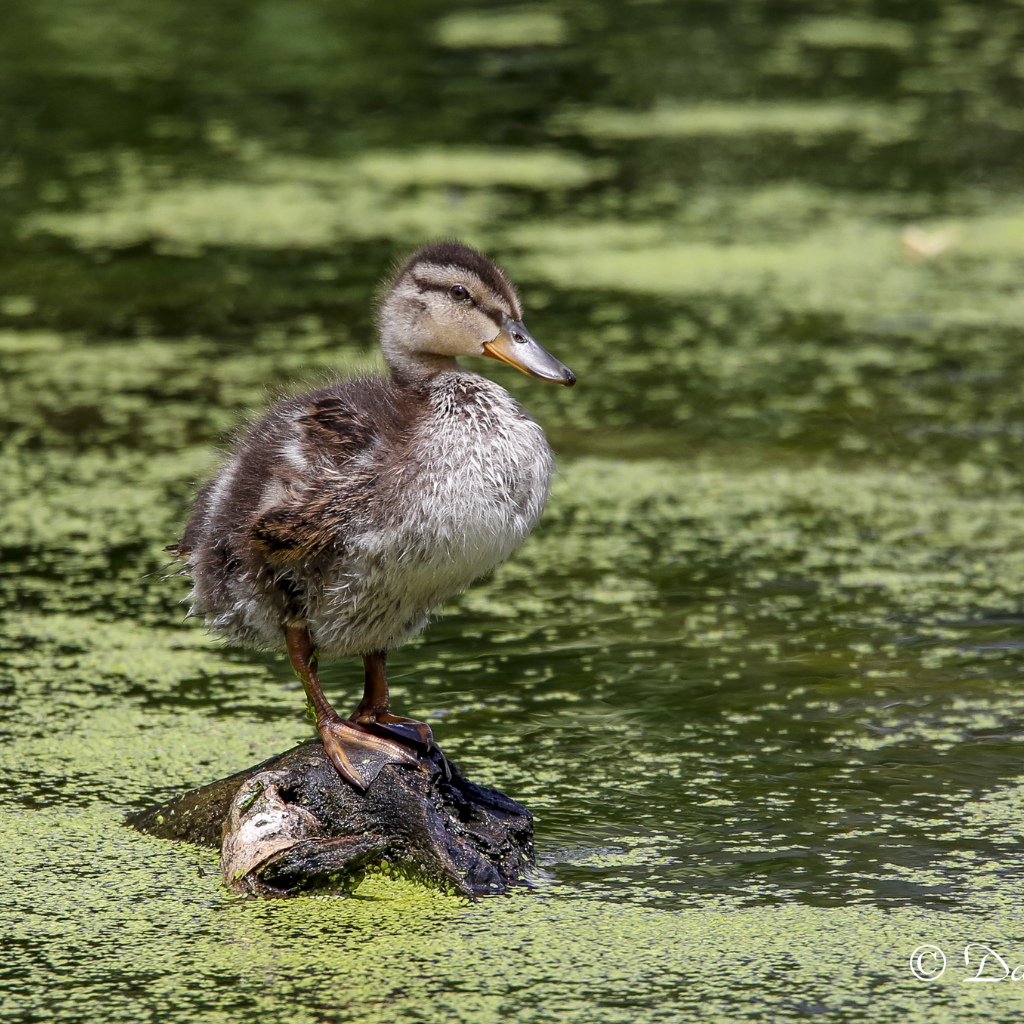
\includegraphics[width=\textwidth]{duck_clean.png}
        \captionof{figure}{Original Image}
    \end{column}
    
    \begin{column}{0.48\textwidth}
        \centering
        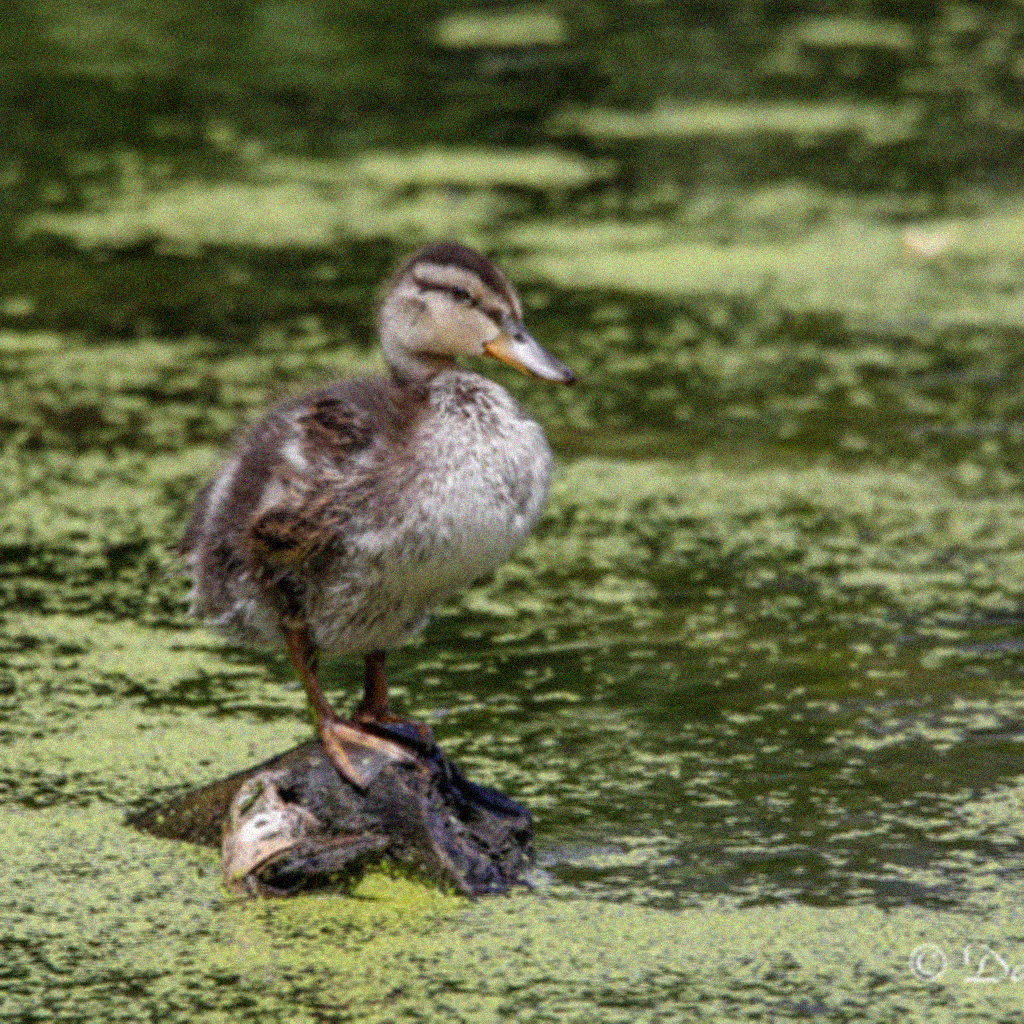
\includegraphics[width=\textwidth]{duck_noisy.png}
        \captionof{figure}{Noisy Image ($\sigma_b = 10, \sigma_n = 15$)}
    \end{column}
\end{columns}

\end{frame}




\section{Methods}

\begin{frame}{Analytical method: Denoise and Deblur}
    \textbf{} A sequential approach to prevent the exponential noise amplification typical of iterative deblurring methods.

    \vspace{0.3cm}
    \textbf{Algorithm Architecture:}
    \begin{enumerate}
        \item \textbf{Spatial Denoising}
        \begin{itemize}
            \item Bilateral Filter to attenuate high-frequency noise.
            \item Preserves geometric structures and sharp edges ($d=9, \sigma_{color}=75, \sigma_{space}=75$).
        \end{itemize}
        
        \vspace{0.15cm}
        \item \textbf{Iterative Deblurring}
        \begin{itemize}
            \item Richardson-Lucy algorithm (Non-Blind solution).
            \item Multiplicative update equation using the spatially inverted kernel ($K^T$):
            \begin{equation*}
                x_{t+1} = x_t \cdot \left( \frac{y}{x_t * K} * K^T \right)
            \end{equation*}
            \item Applies \textit{reflect padding} to eliminate boundary artifacts.
        \end{itemize}
    \end{enumerate}

    % \vspace{0.3cm}
    % \begin{block}{Validated Performance}
    %     Evaluation on the Flickr2K dataset: \textbf{Average PSNR = 25.96 dB}. \\
    %     Serves as a classical baseline for evaluating Deep Learning models.
    % \end{block}
\end{frame}

\begin{frame}{Deep Learning Approach: DnCNN Architecture}
    \textbf{} The Denoising Convolutional Neural Network (DnCNN) is a milestone architecture that established Deep Learning as the standard for image restoration.

    \vspace{0.3cm}
    \textbf{Innovations:}
    \begin{itemize}
        \item \textbf{Residual Learning Formulation:} Instead of outputting the clean image directly, the network is trained to predict the residual image. 
        \begin{equation*}
            \text{Clean Image} = \text{Degraded Image} - \text{Predicted Noise}
        \end{equation*}
        \item \textbf{Batch Normalization (BN):} Integration of BN with ReLU activation functions accelerates the training process and boosts overall performance.
        \item \textbf{} It maintains the original image dimensions throughout all convolutional layers, preventing the loss of fine spatial details.
    \end{itemize}
\end{frame}

\begin{frame}{DnCNN: Advantages for Denoising \& Deblurring}
    \textbf{Why use DnCNN?}

    \vspace{0.3cm}
    \begin{itemize}
        \item \textbf{}Capable of both denoise and deblur at the same time
        \item \textbf{Blind Denoising:} Can be trained to handle a wide range of noise levels simultaneously, without requiring the exact noise variance ($\sigma$) as an input parameter.
        \item \textbf{}It serves as the perfect intermediate benchmark, outperforming traditional filters while offering a simple, linear architecture.
    \end{itemize}

    % \vspace{0.3cm}
    % \begin{block}{Expected Impact}
    %     Provides a highly stable restoration, significantly improving the PSNR compared to the 25.96 dB classical baseline, specifically by eliminating granular noise without blurring sharp edges.
    % \end{block}
\end{frame}

\begin{frame}{DnCNN}
\begin{figure}
    \centering
    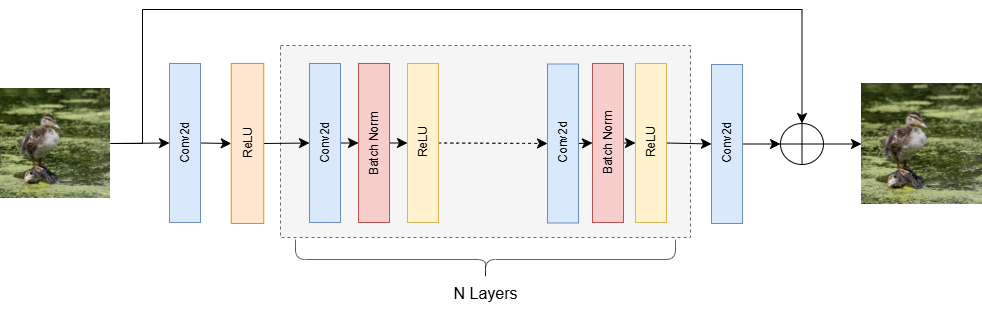
\includegraphics[width=1\textwidth]{dncnn.drawio.png}
    \caption{DnCNN Arhitecture}
\end{figure}
\textbf{Conv2d:} 64 filters with 3x3 kernel
\end{frame}



\begin{frame}{Deep Learning Approach: ResUNet Architecture}
    \textbf{} A hybrid architecture that integrates Residual Networks into a U-Net backbone.

    \vspace{0.3cm}
    \textbf{Components:}
    \begin{itemize}
        \item \textbf{Encoder-Decoder Structure:} 
        \begin{itemize}
            \item \textit{Encoder:} Progressively downsamples the image to extract deep, multi-scale feature representations.
            \item \textit{Decoder:} Upsamples the features to reconstruct the image at its original resolution.
        \end{itemize}
        
        \item \textbf{Skip Connections:} Directly transfer spatial details from the encoder to the decoder, preventing the loss of fine textures.
        
        \item \textbf{Residual Blocks:} Replace standard convolutional layers. They utilize shortcut connections to bypass layers, mitigating the vanishing gradient problem and allowing for deeper networks.
    \end{itemize}
\end{frame}

\begin{frame}{ResUNet: Advantages for Denoising \& Deblurring}
    \textbf{Why it outperforms classical methods:}

    \vspace{0.3cm}
    \begin{itemize}
        \item \textbf{Residual Learning:} Instead of mapping the degraded image directly to a clean image, the network learns to predict the residual (the noise and blur components). This simplifies the optimization process.
        \item \textbf{Global Context vs. Local Detail:} The multi-scale nature of the U-Net handles large blur kernels (global context) while skip connections restore sharp geometric edges (local detail).
        \item \textbf{Blind Restoration:} It infers the degradation pattern from the data distribution.
    \end{itemize}

    % \vspace{0.3cm}
    % \begin{block}{Expected Performance Shift}
    %     Deep learning models like ResUNet typically achieve \textbf{$> 30$ dB PSNR} on high-resolution datasets, representing a massive quantitative and qualitative leap over the $25.96$ dB classical baseline.
    % \end{block}
\end{frame}

\begin{frame}{ResUNet}
\begin{figure}
    \centering
    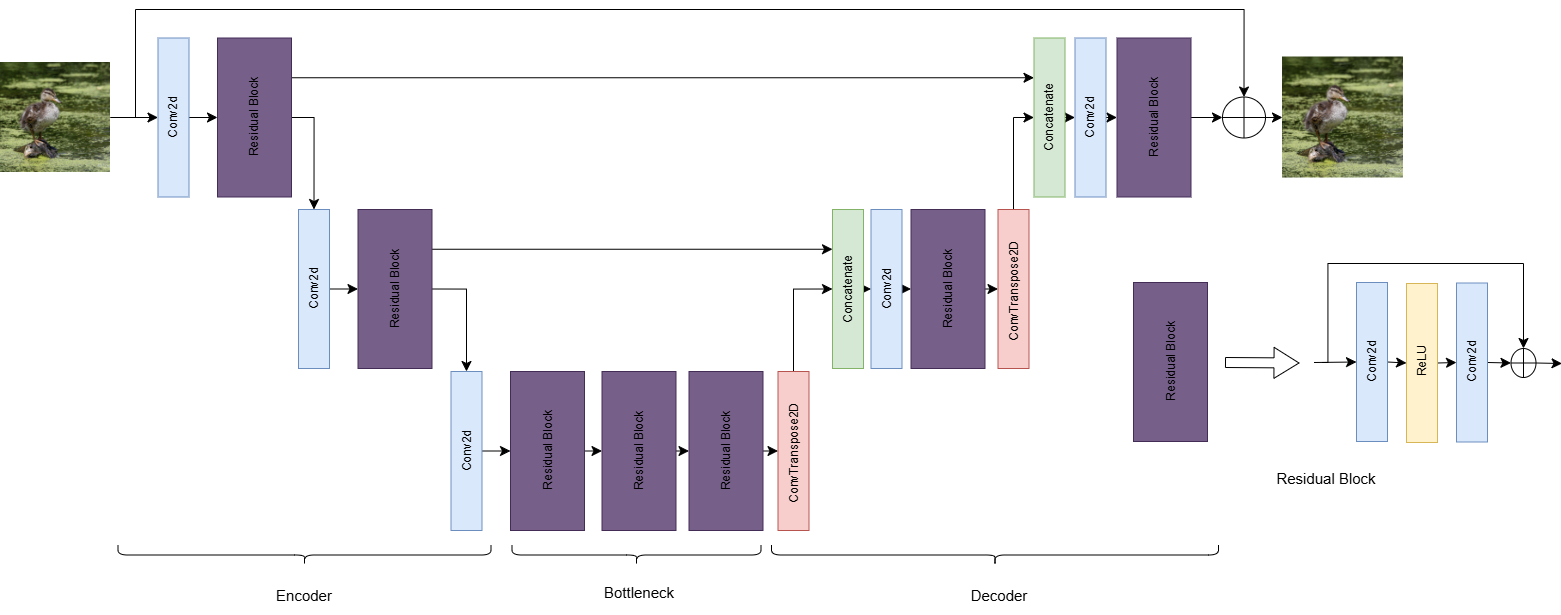
\includegraphics[width=1\textwidth]{Res_U-net.drawio.png}
    \caption{Residual U-Net Arhitecture}
\end{figure}
\end{frame}

\begin{frame}{Uformer: SOTA Reference Model (Pre-trained)}
    \textbf{} Advanced Vision Transformer architecture as a State-of-the-Art benchmark.

    \vspace{0.3cm}
    \textbf{Key Features:}
    \begin{itemize}
        \item \textbf{} Replaces classic convolutions with Window-based Self-Attention mechanisms.
        \item \textbf{} The attention mechanism allows it to correlate pixels in opposite corners of the image, making it highly effective for extensive degradations.
        \item \textbf{} Retains the U-Net arhitecture (Encoder-Decoder with skip connections) to prevent the loss of spatial details.
    \end{itemize}
\end{frame}

\begin{frame}{Restormer: SOTA Benchmark (Pre-trained)}
    \textbf{} Cutting-edge Vision Transformer model as an absolute performance reference.

    \vspace{0.3cm}
    \textbf{Key Features:}
    \begin{itemize}
        \item \textbf{} Unlike standard Transformers, it processes full-resolution images natively, eliminating boundary artifacts.
        \item \textbf{} Extracts global context by analyzing correlations across feature channels, making it highly effective for severe motion blur.
        \item \textbf{} Combines the global analysis of a Transformer with the local precision of convolutions to restore fine textures clearly.
    \end{itemize}

    % \vspace{0.3cm}
    % \begin{block}{Role in the Project}
    %     Similar to Uformer, it acts as the \textbf{theoretical upper bound}. As a top-tier pre-trained model, it provides the ultimate benchmark to evaluate the efficiency and limits of the locally trained networks (DnCNN, ResUNet).
    % \end{block}
\end{frame}

\begin{frame}{Experimental Setup and Training Methodology}
    \vspace{0.2cm}
    \begin{columns}[T]
        
        % Left Column
        \begin{column}{0.5\textwidth}
            \textbf{Hyperparameters}
            \begin{itemize}
                \item \textbf{Epochs:} 10
                \item \textbf{Batch Size:} 16
                \item \textbf{Optimizer:} Adam
                \item \textbf{Learning Rate:} 0.001 (0.0001 for ResUNet)
            \end{itemize}
            
            \vspace{0.4cm}
            \textbf{Pipeline Reliability}
            \begin{itemize}
                \item \textbf{Checkpointing:} Saving the best-performing model weights.
                \item \textbf{Fault Tolerance:} Continuous state backups allowing training resumption in case of interruption.
            \end{itemize}
        \end{column}
        
        % Right Column
        \begin{column}{0.5\textwidth}
            \textbf{Objective Functions \& Evaluation}
            \begin{itemize}
                \item \textbf{Loss Configurations:}
                \begin{itemize}
                    \item Standard: MSE
                    \item Hybrid 1: 0.8 MAE + 0.2 MSE
                    \item Hybrid 2: 0.8 MAE + 0.2 SSIM
                \end{itemize}
                
                \vspace{0.2cm}
                \item \textbf{Evaluation Metrics:} 
                \begin{itemize}
                    \item PSNR \& MSE
                \end{itemize}

                \vspace{0.2cm}
                \item \textbf{Group 5-Fold Cross-Validation:} 
                \begin{itemize}
                    \item Applied during subset testing.
                \end{itemize}
            \end{itemize}
        \end{column}

    \end{columns}
\end{frame}

%===================================================================================================
% Results
%===================================================================================================

\section{Results}

\begin{frame}{Loss Function Comparison}
    \vspace{0.2cm}
    
    \begin{table}[]
        \centering
        \renewcommand{\arraystretch}{1.3}
        \begin{tabular}{lcc}
            \toprule
            \textbf{Loss Configuration} & \textbf{PSNR (dB)} & \textbf{MSE} \\
            \midrule
            MSE                 & 28.38 & 0.0021 \\
            0.8 MAE + 0.2 MSE   & 28.54 & 0.0020 \\
            0.8 MAE + 0.2 SSIM  & 28.45 & 0.0021 \\
            \bottomrule
        \end{tabular}
    \end{table}
    \textbf{Setup:} ResUNet with k-fold trained on a subset of 100 images

    \vspace{0.4cm}
    \begin{itemize}
        \item \textbf{MSE Baseline:} Maximizes PSNR but over-smooths textures and loses high-frequency details.
        \item \textbf{MAE + MSE:} MAE preserves sharp edges and handles outliers; MSE reduces overall variance.
        \item \textbf{MAE + SSIM:} Optimizes for human visual perception by prioritizing structural integrity over pixel intensity.
    \end{itemize}
\end{frame}

\begin{frame}{Loss Function Comparison: Convergence Plots}
    \vspace{0.1cm}
    
    % Rândul 1 (Sus)
    \begin{columns}[T]
        \begin{column}{0.48\textwidth}
            \centering
            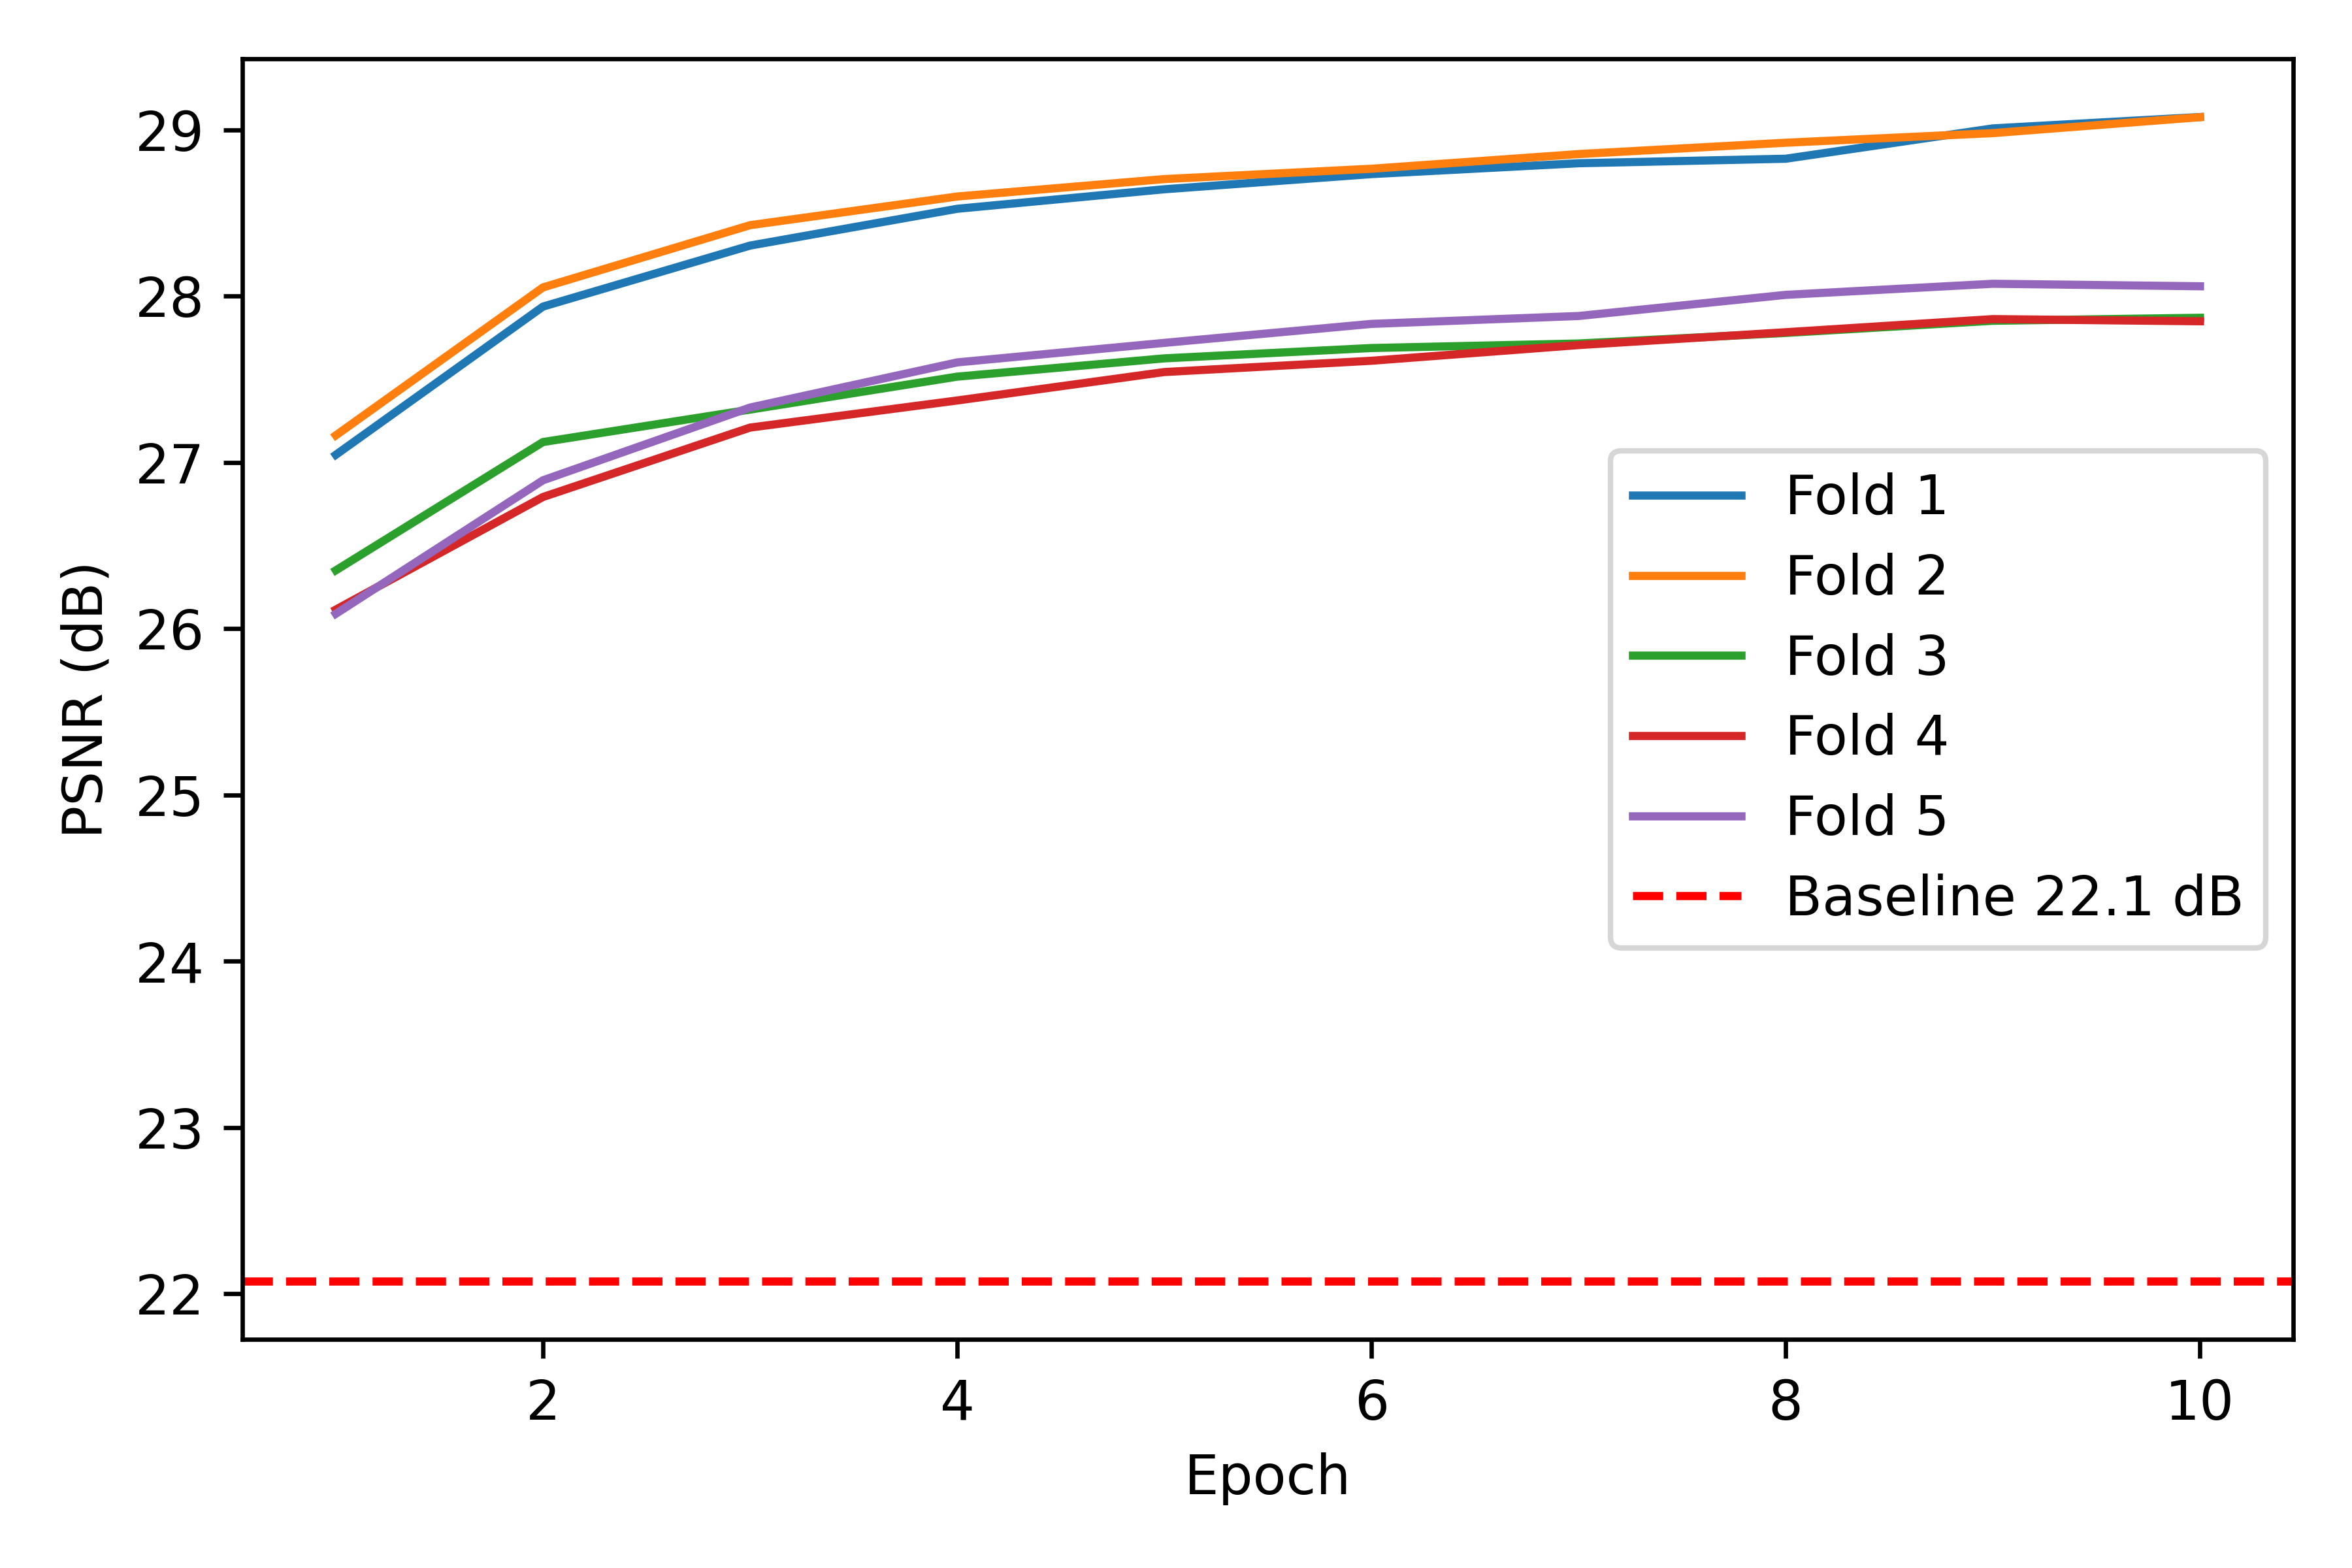
\includegraphics[width=0.8\linewidth]{Plot_PSNR_LOSS_MSE.png}
            \vspace{0.1cm} \\
            \small \textbf{MSE} \\
        \end{column}
        \begin{column}{0.48\textwidth}
            \centering
            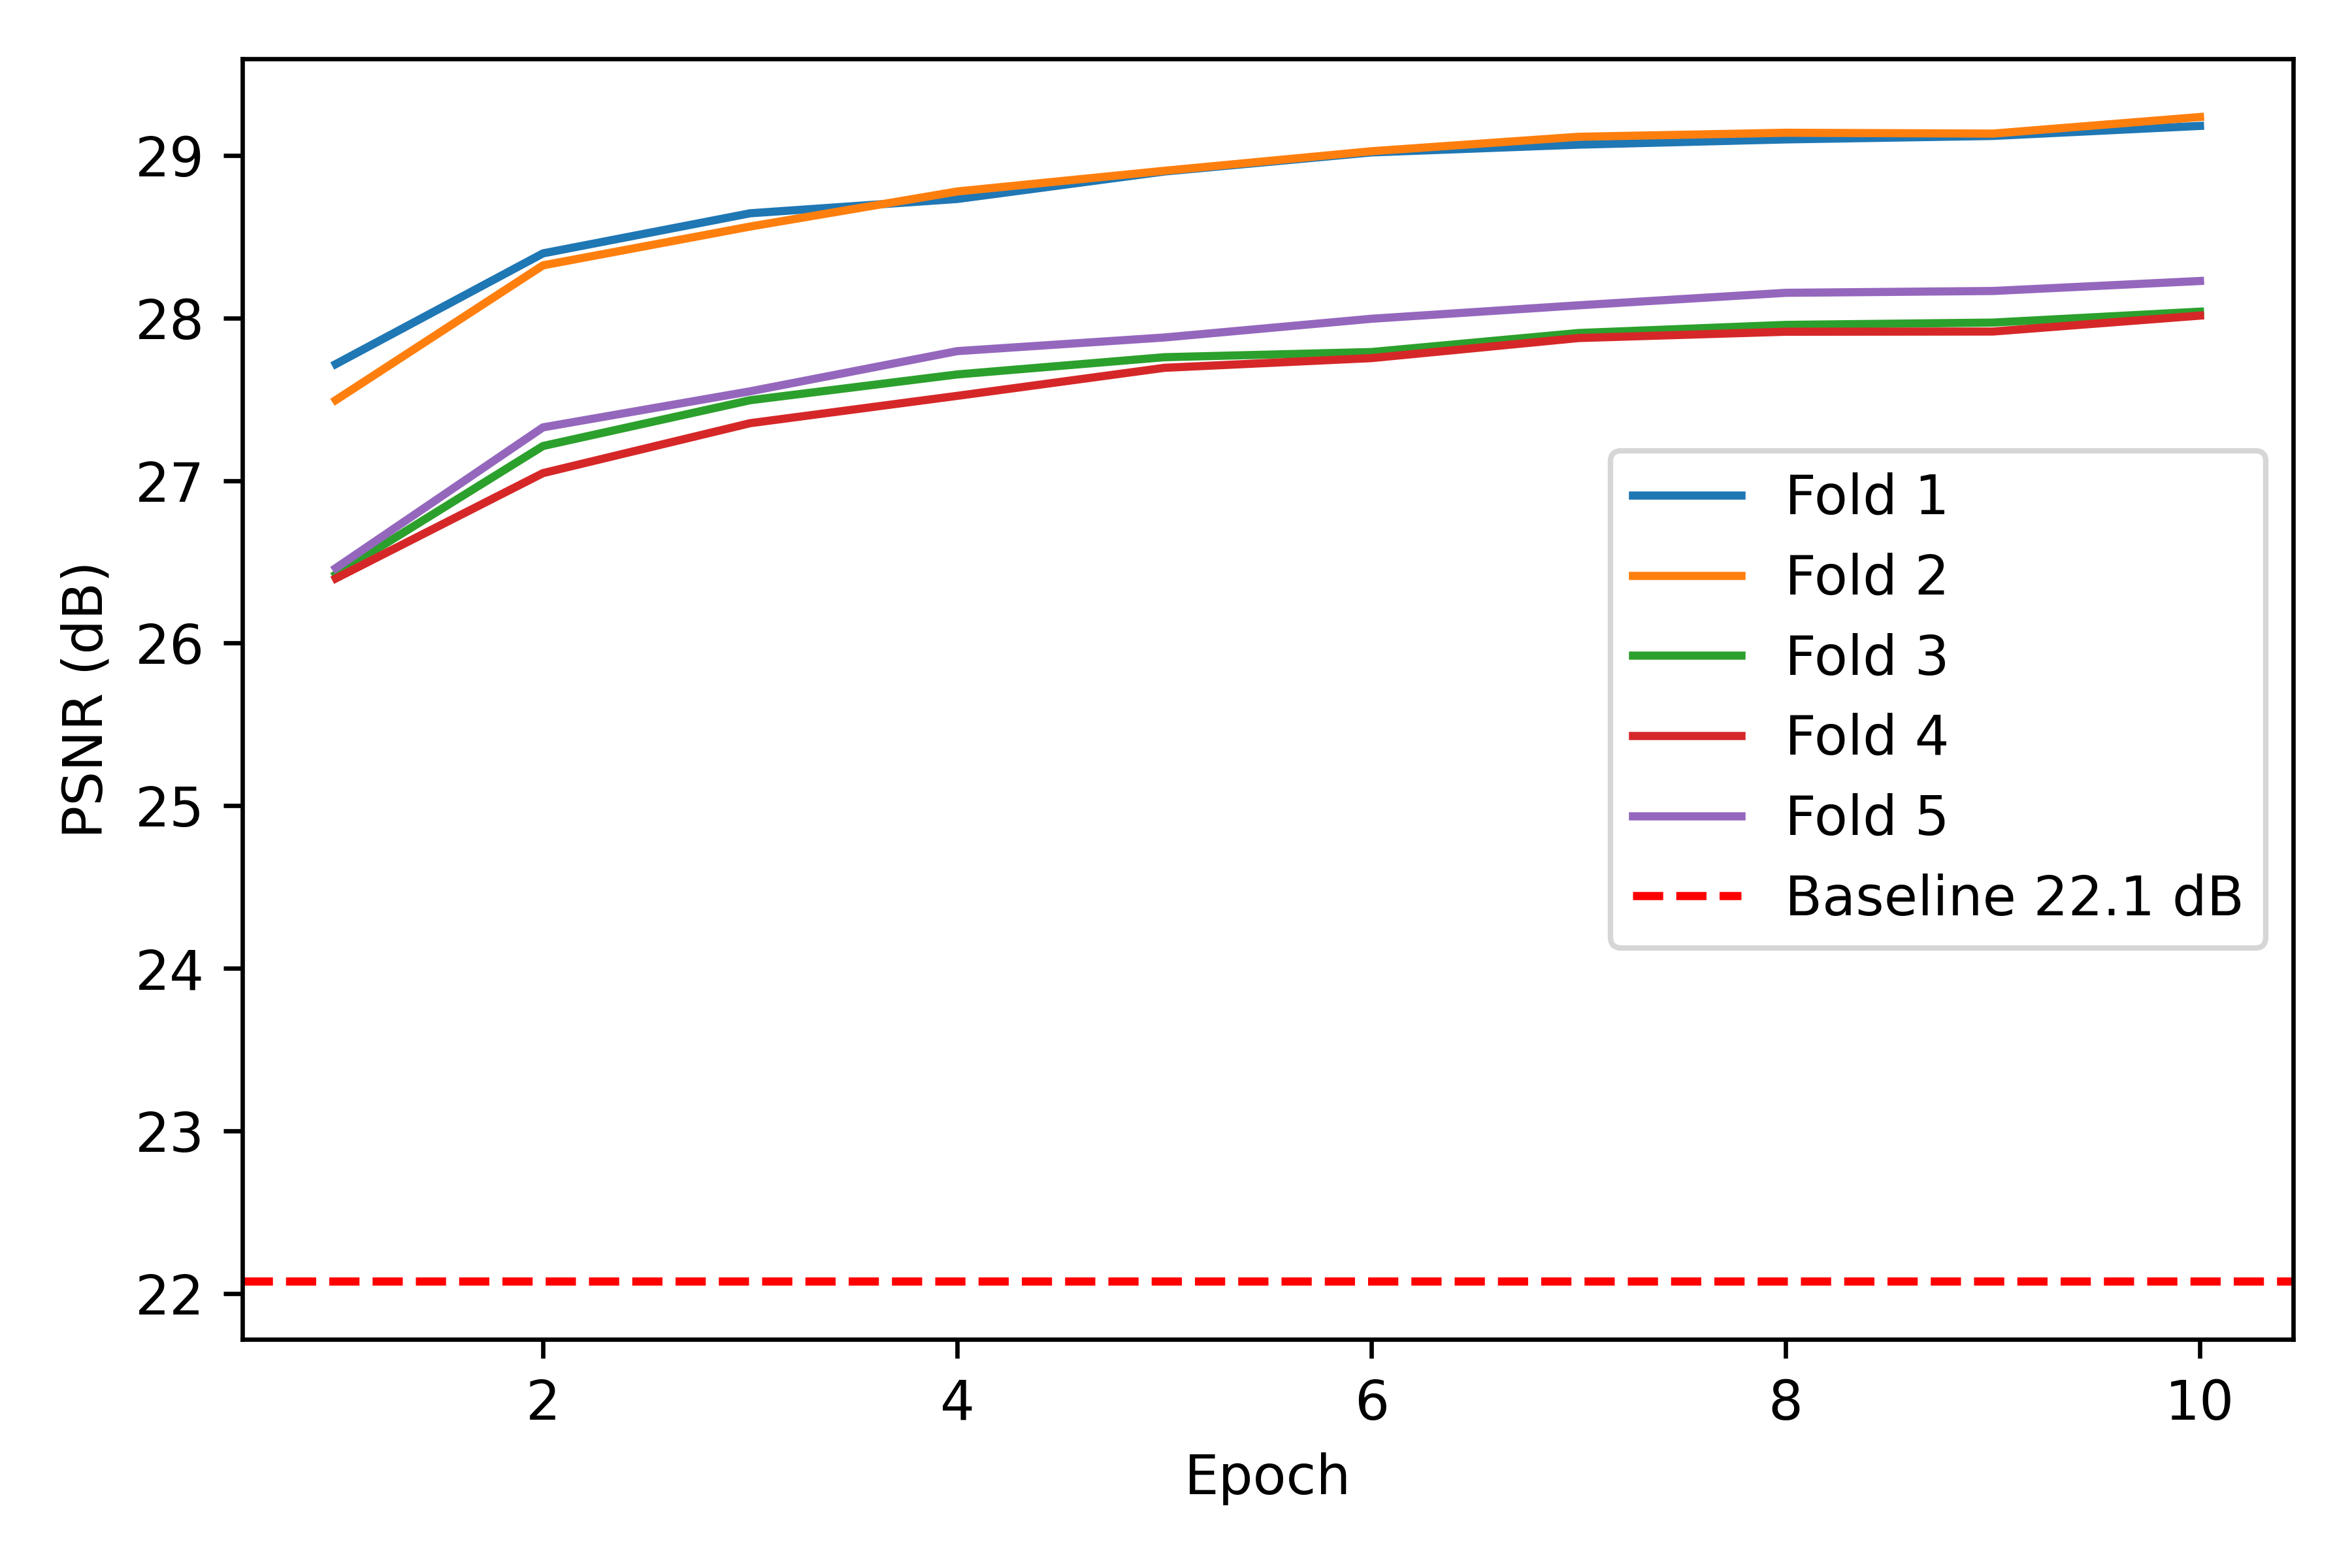
\includegraphics[width=0.8\linewidth]{Plot_PSNR_LOSS_MAE+MSE.png}
            \vspace{0.1cm} \\
            \small \textbf{MAE + MSE} \\
        \end{column}
    \end{columns}

    \vspace{0.3cm}
    
    % Rândul 2 (Jos)
    \begin{columns}[T]
        \begin{column}{0.48\textwidth}
            \centering
            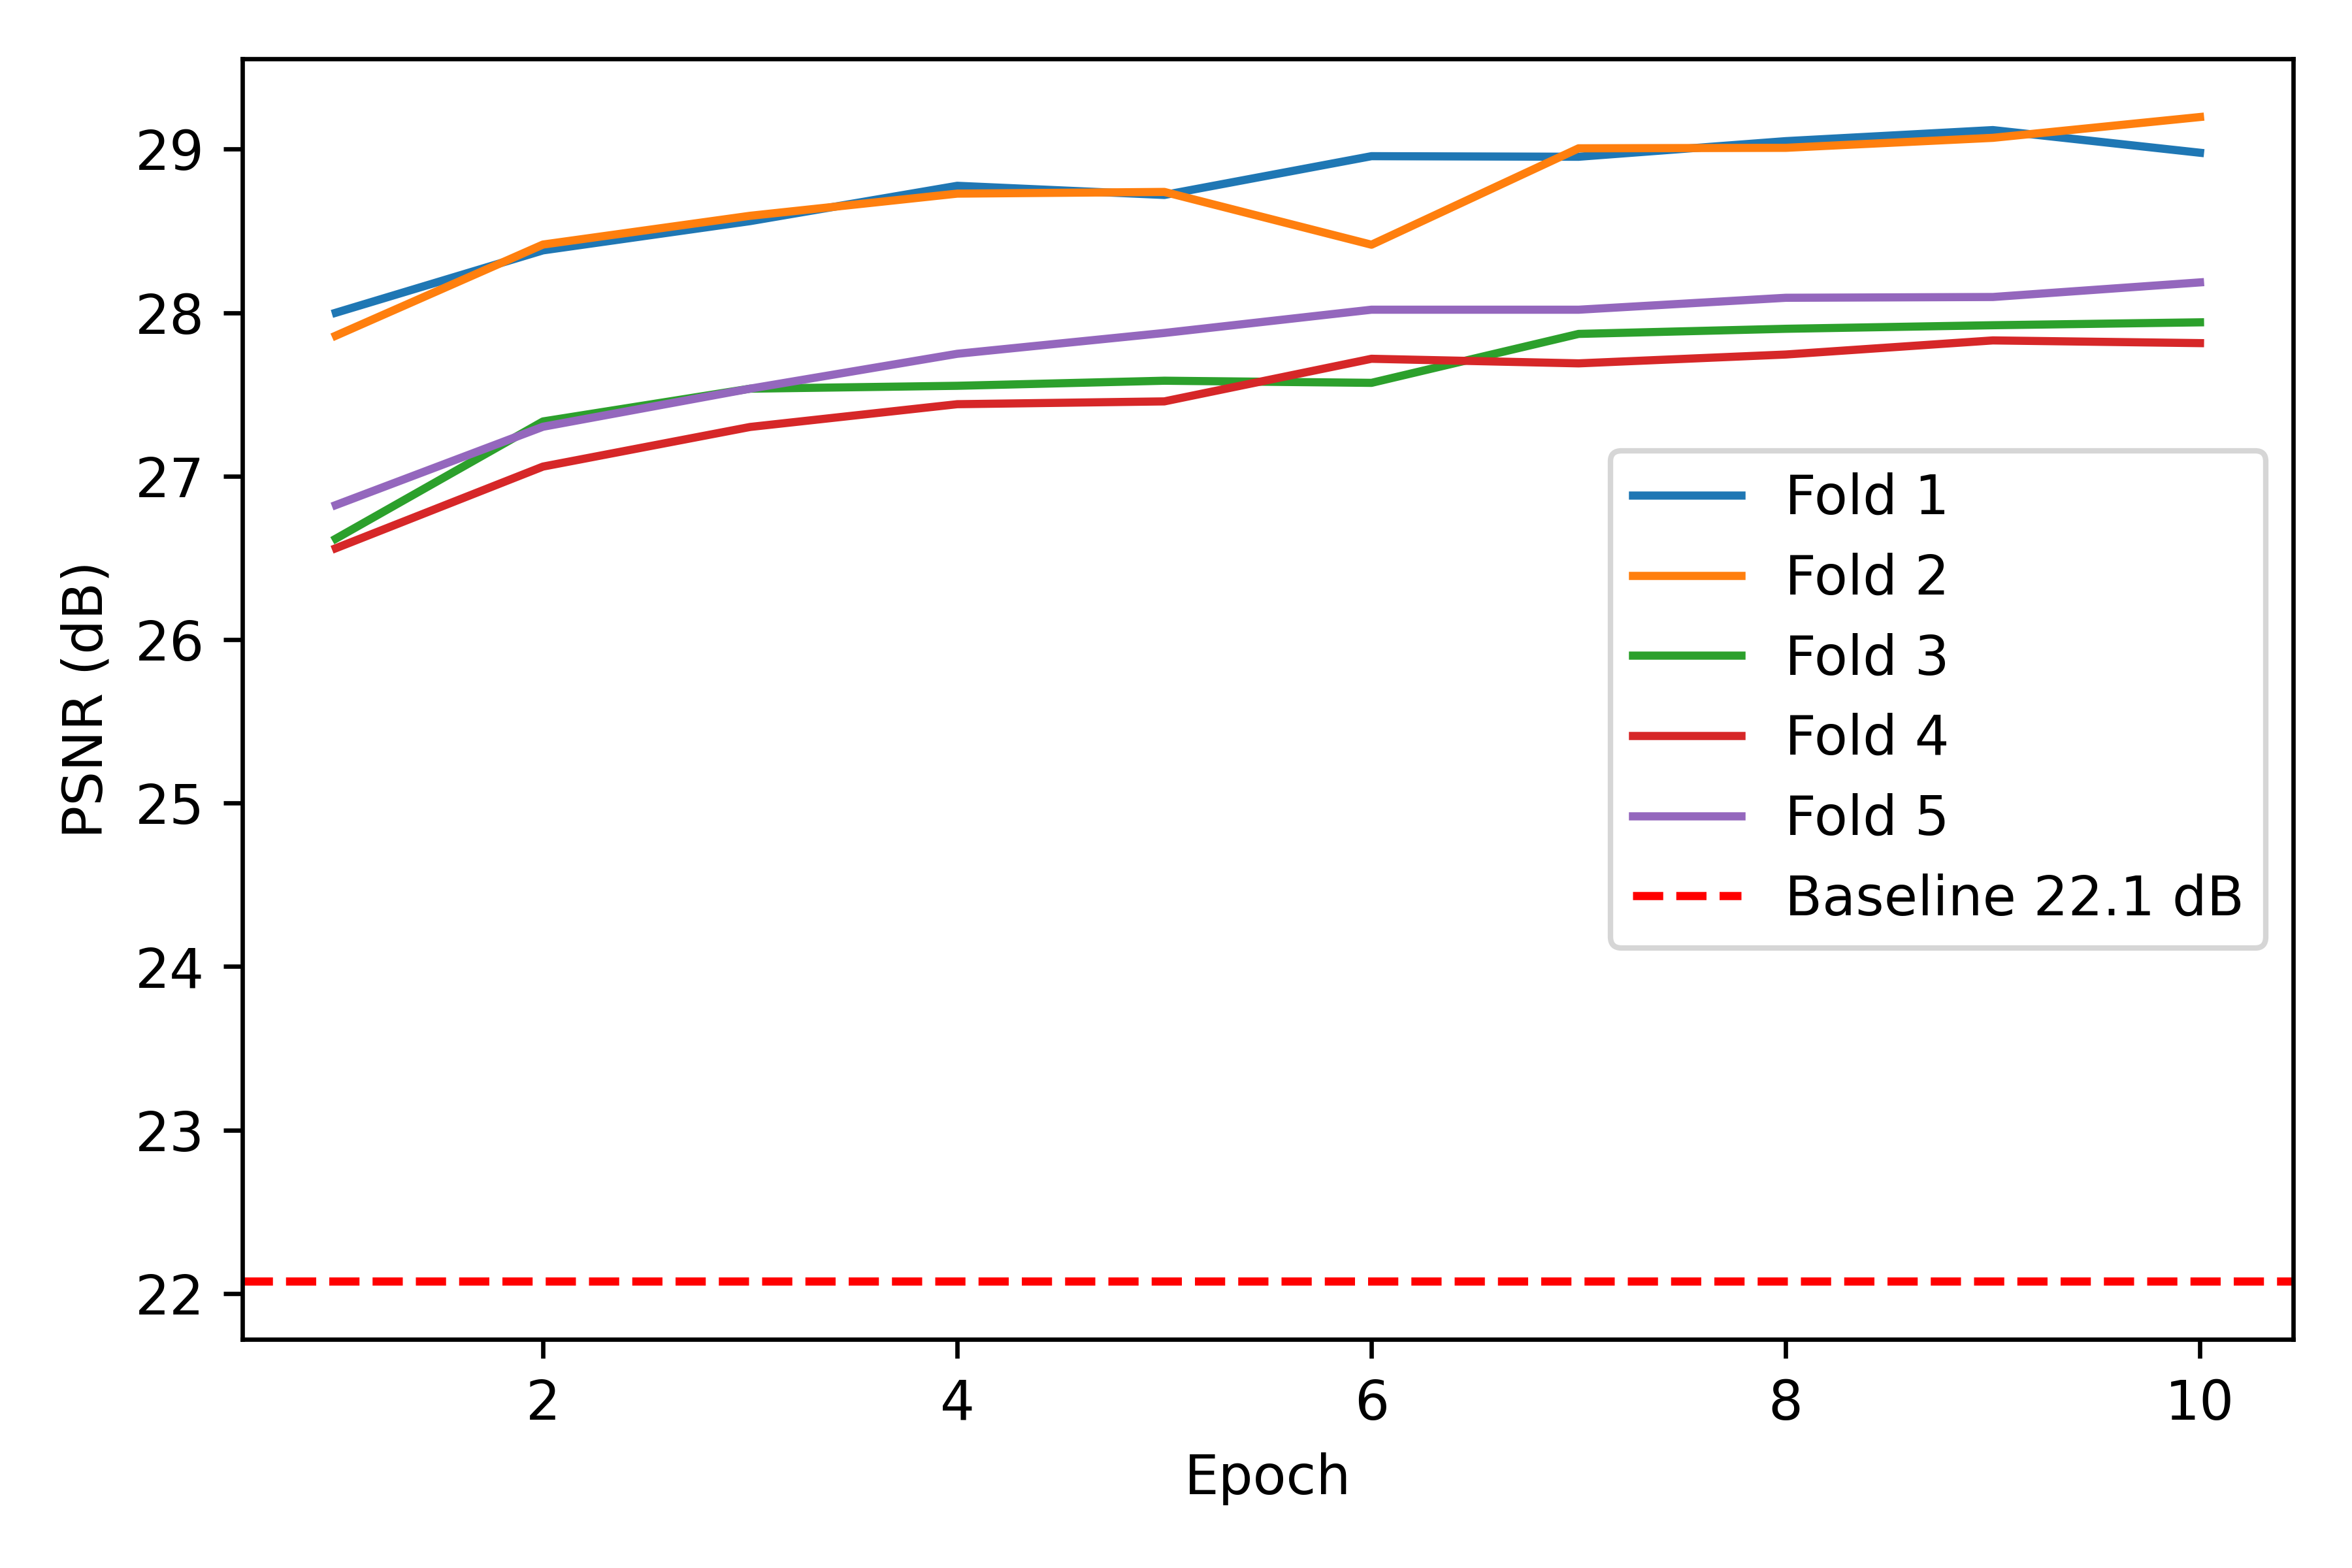
\includegraphics[width=0.8\linewidth]{Plot_PSNR_LOSS_MAE+SSIM.png}
            \vspace{0.1cm} \\
            \small \textbf{MAE + SSIM} \\
        \end{column}
        \begin{column}{0.48\textwidth}
            \vspace{0.5cm}
            \begin{block}{Observation}
                % Combining MAE with auxiliary loss terms stabilizes training, preventing the rapid overfitting observed with pure MSE.
            \end{block}
        \end{column}
    \end{columns}
\end{frame}

\begin{frame}{Model Trained with MSE}
\begin{figure}
    \centering
    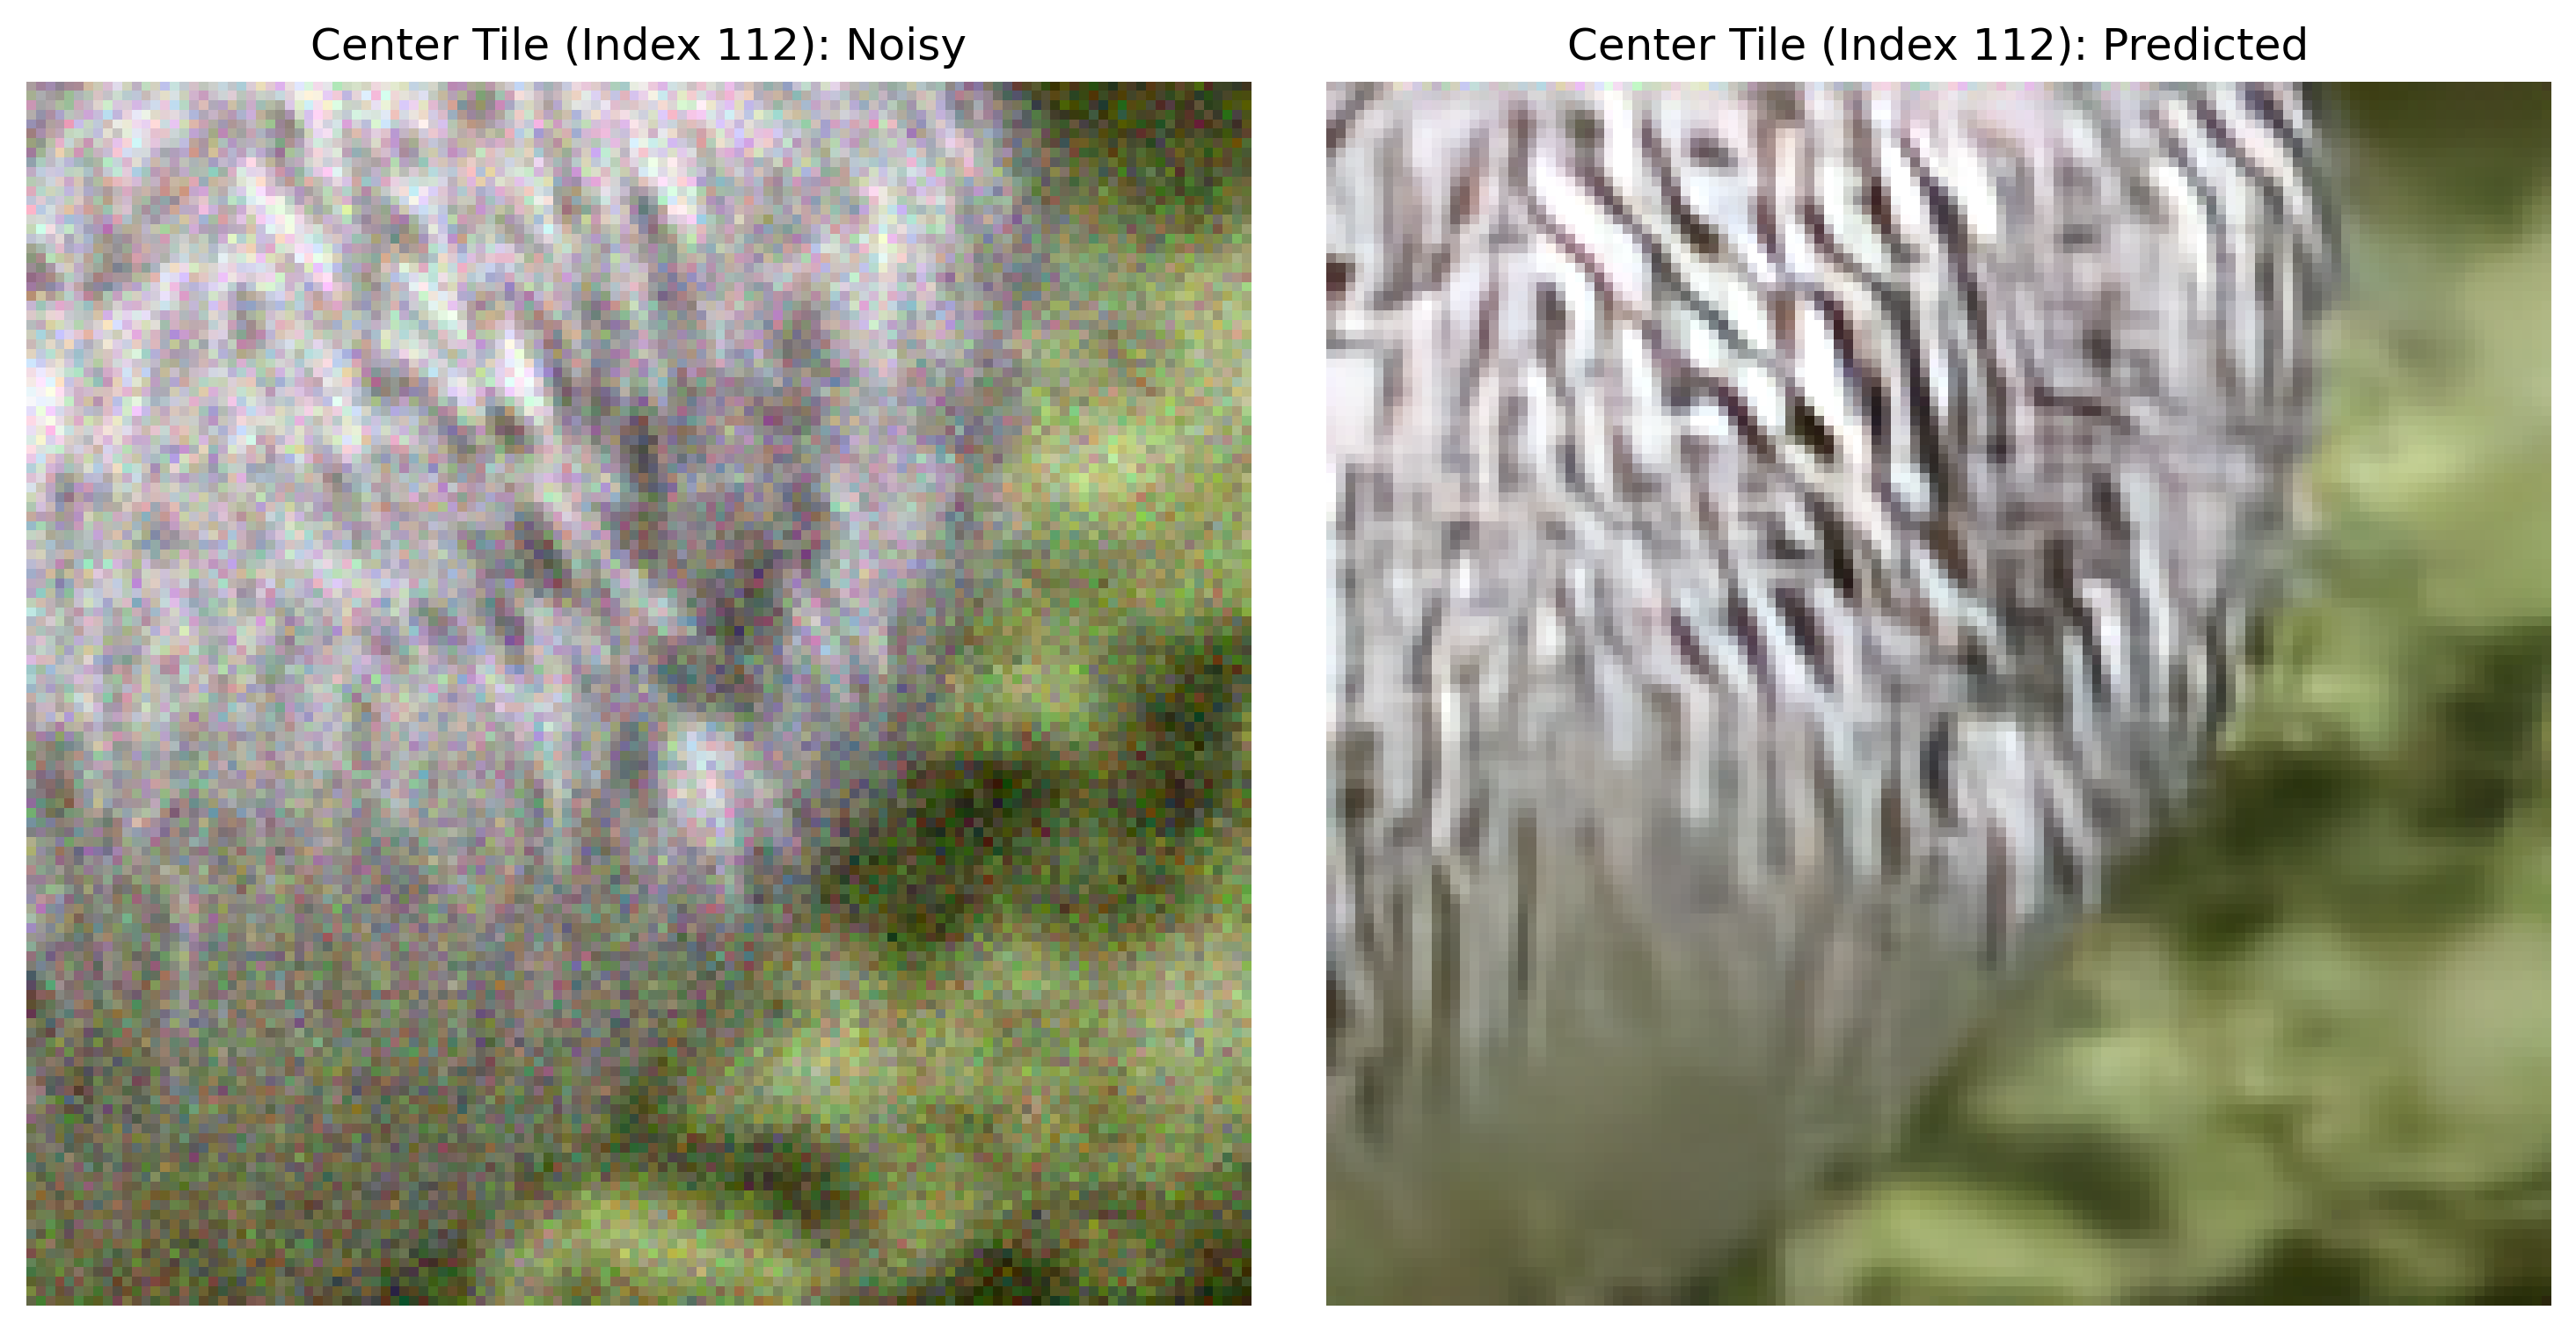
\includegraphics[width=1\textwidth]{duck_DnCNN_Full_CenterTile.png}
\end{figure}
\end{frame}

\begin{frame}{Model Trained with MAE + SSIM}
\begin{figure}
    \centering
    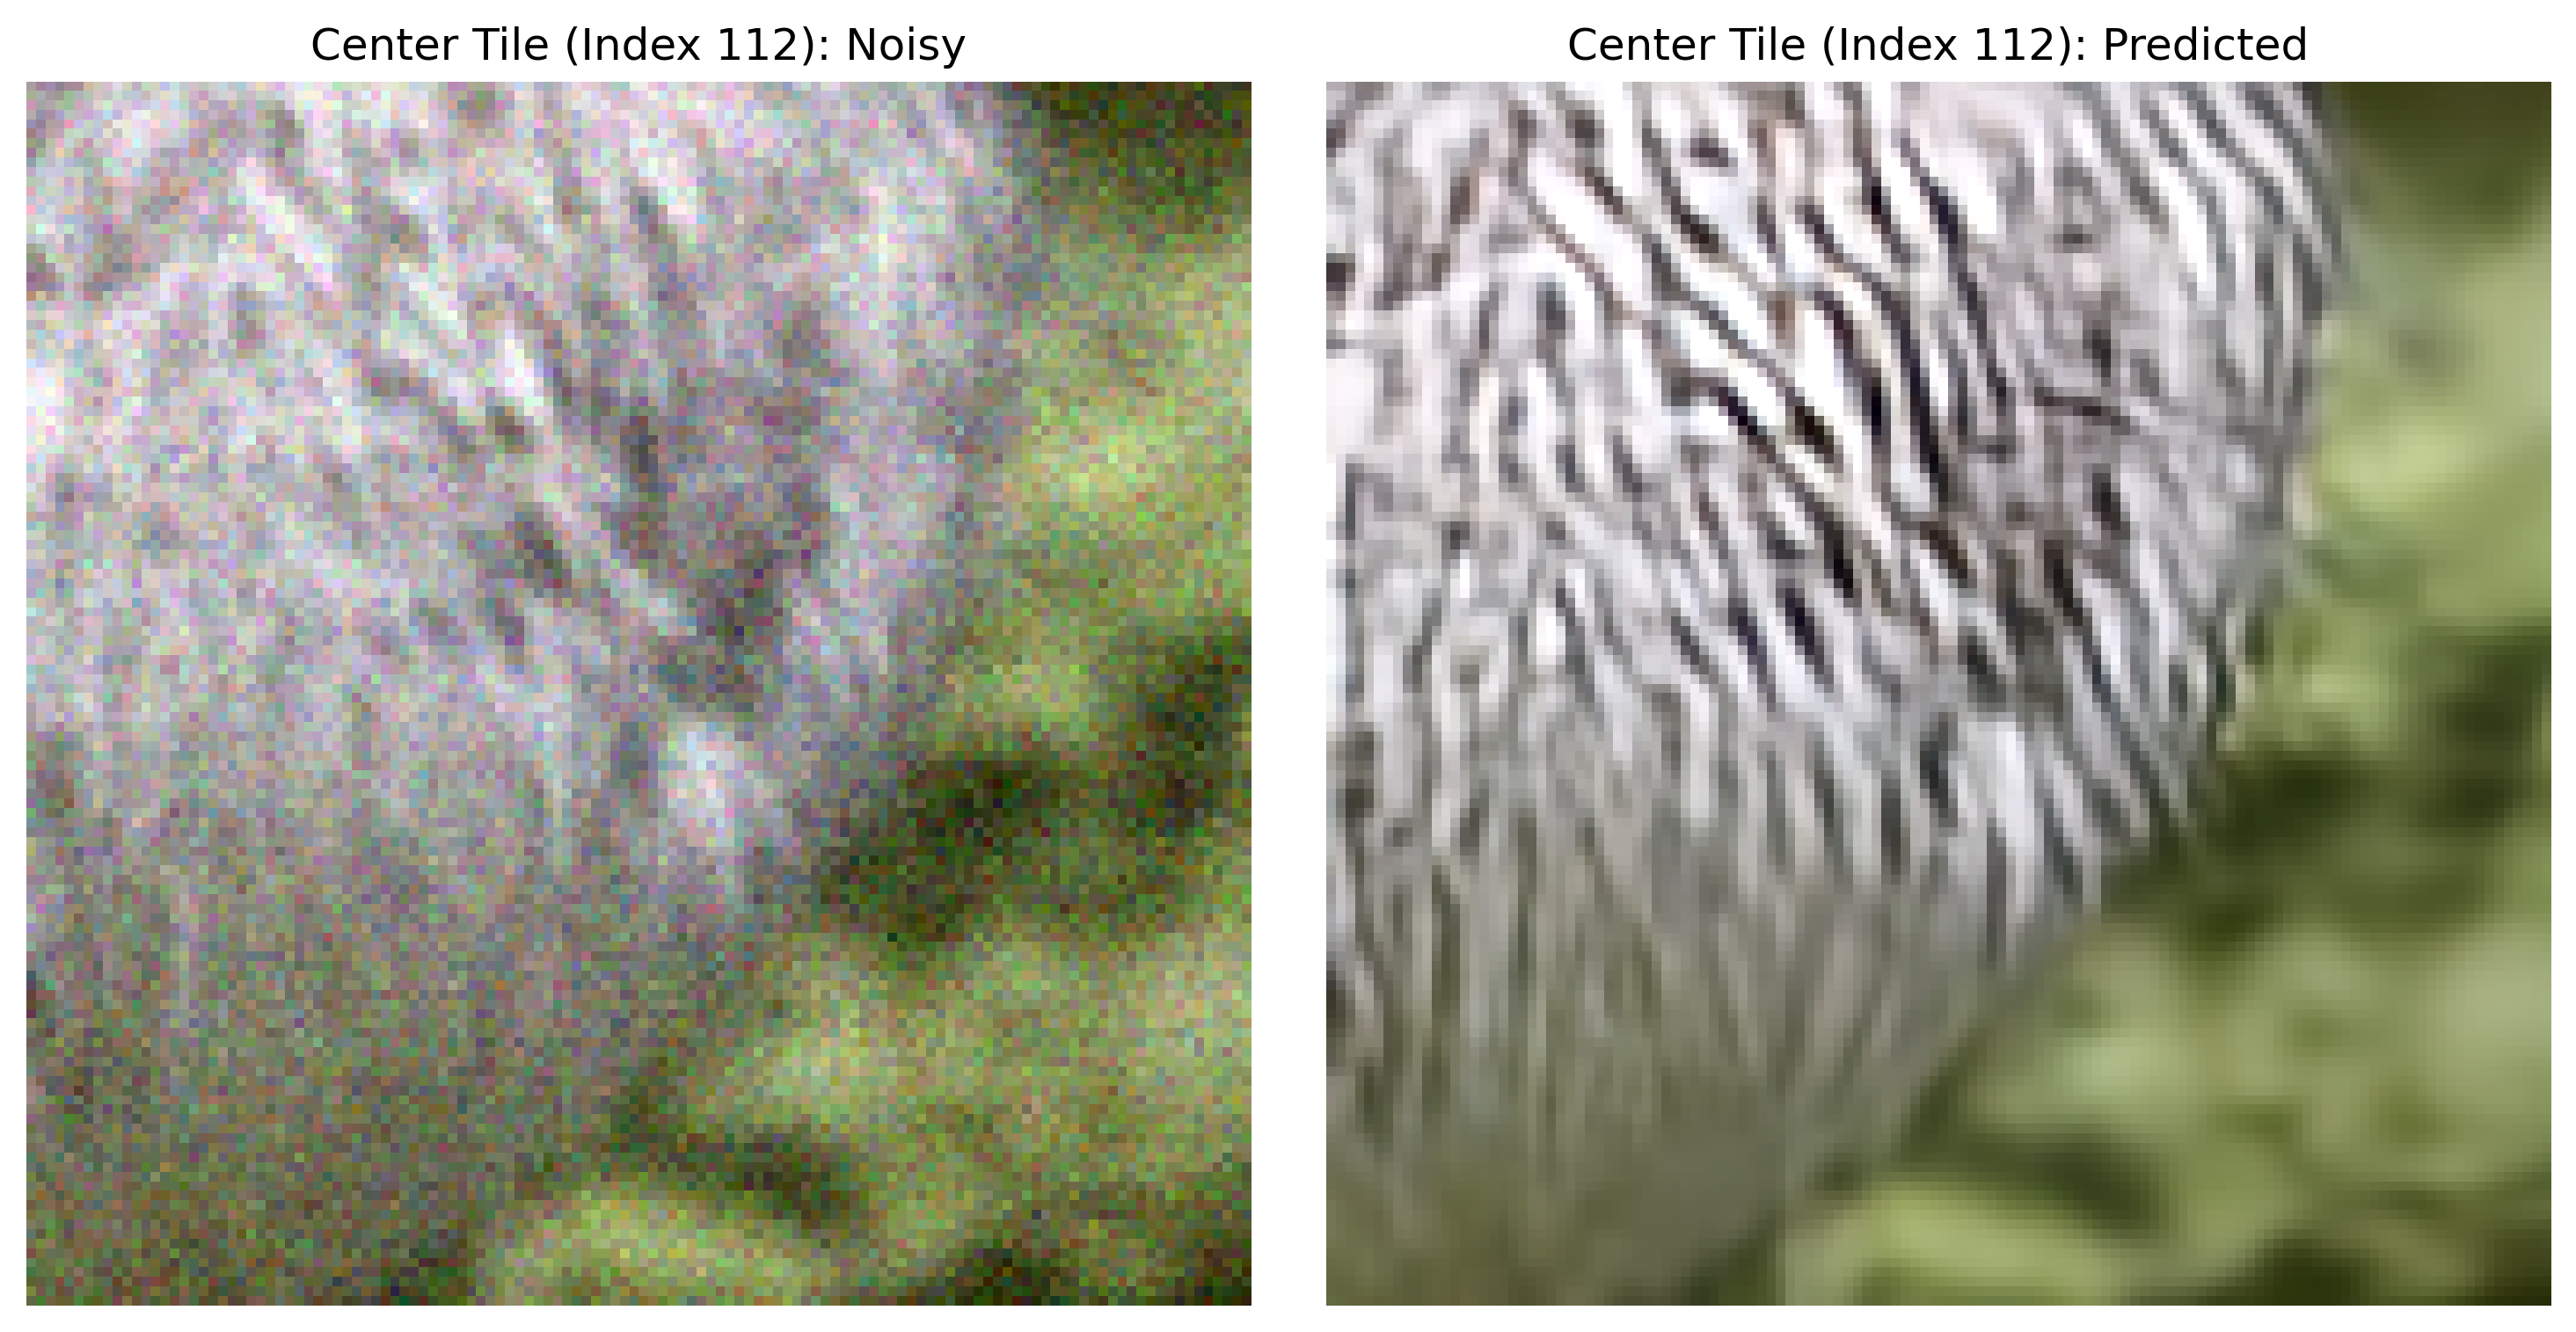
\includegraphics[width=1\textwidth]{duck_ResUNet_Full_CenterTile.png}
\end{figure}
\end{frame}

\begin{frame}{DnCNN}
\begin{figure}
    \centering
    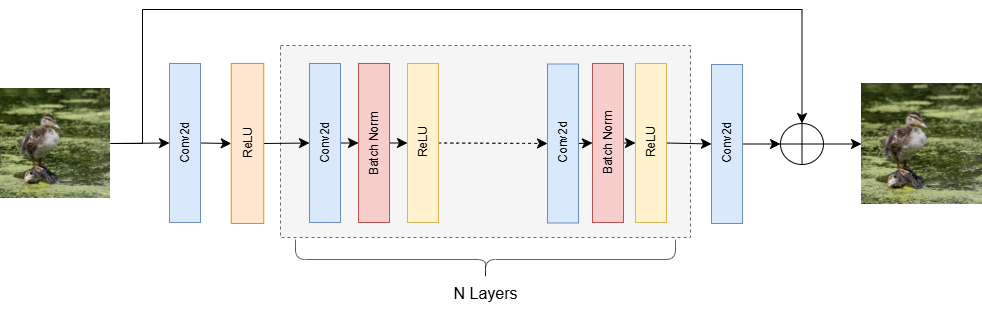
\includegraphics[width=1\textwidth]{dncnn.drawio.png}
    \caption{DnCNN Arhitecture}
\end{figure}
\textbf{Conv2d:} 64 filters with 3x3 kernel
\end{frame}

\begin{frame}{Comparative Analysis of Proposed Methods}
    \vspace{0.2cm}
    
    \begin{table}[]
        \centering
        \renewcommand{\arraystretch}{1.3}
        \resizebox{\textwidth}{!}{%
        \begin{tabular}{llccc}
            \toprule
            \textbf{Method} & \textbf{Architecture Category} & \textbf{PSNR (dB)} & \textbf{MSE} & \textbf{Loss} \\
            \midrule
            Bilateral + R-Lucy & Analytical         & 25.96 & - & - \\
            DnCNN (MSE, 17 layers)& Linear CNN         & 28.98 & 0.0019 & 0.0019 \\
            ResUNet (MAE+SSIM) & Multi-scale CNN    & 29.22 & 0.0019 & 0.0433 \\
            Uformer            & Vision Transformer & 22.95 & 0.0057 & - \\
            Restormer          & Vision Transformer & XX.XX & 0.XXXX & 0.XXXX \\
            \bottomrule
        \end{tabular}%
        }
    \end{table}
    \textbf{DataSet:} Full mixed variant with $\sigma_b = 10, \sigma_n = 15$

    \vspace{0.4cm}
    \begin{itemize}
        \item \textbf{CNNs vs. Classical:} Deep learning models eliminate the exponential noise amplification inherent to iterative analytical deblurring.
        \item \textbf{ResUNet Efficiency:} The multi-scale approach with skip connections recovers geometric details better than the linear DnCNN.
    \end{itemize}
\end{frame}

\begin{frame}{Proposed Methods Plots}
    \vspace{0.1cm}
    
    % Rândul 1 (Sus)
    \begin{columns}[T]
        \begin{column}{0.48\textwidth}
            \centering
            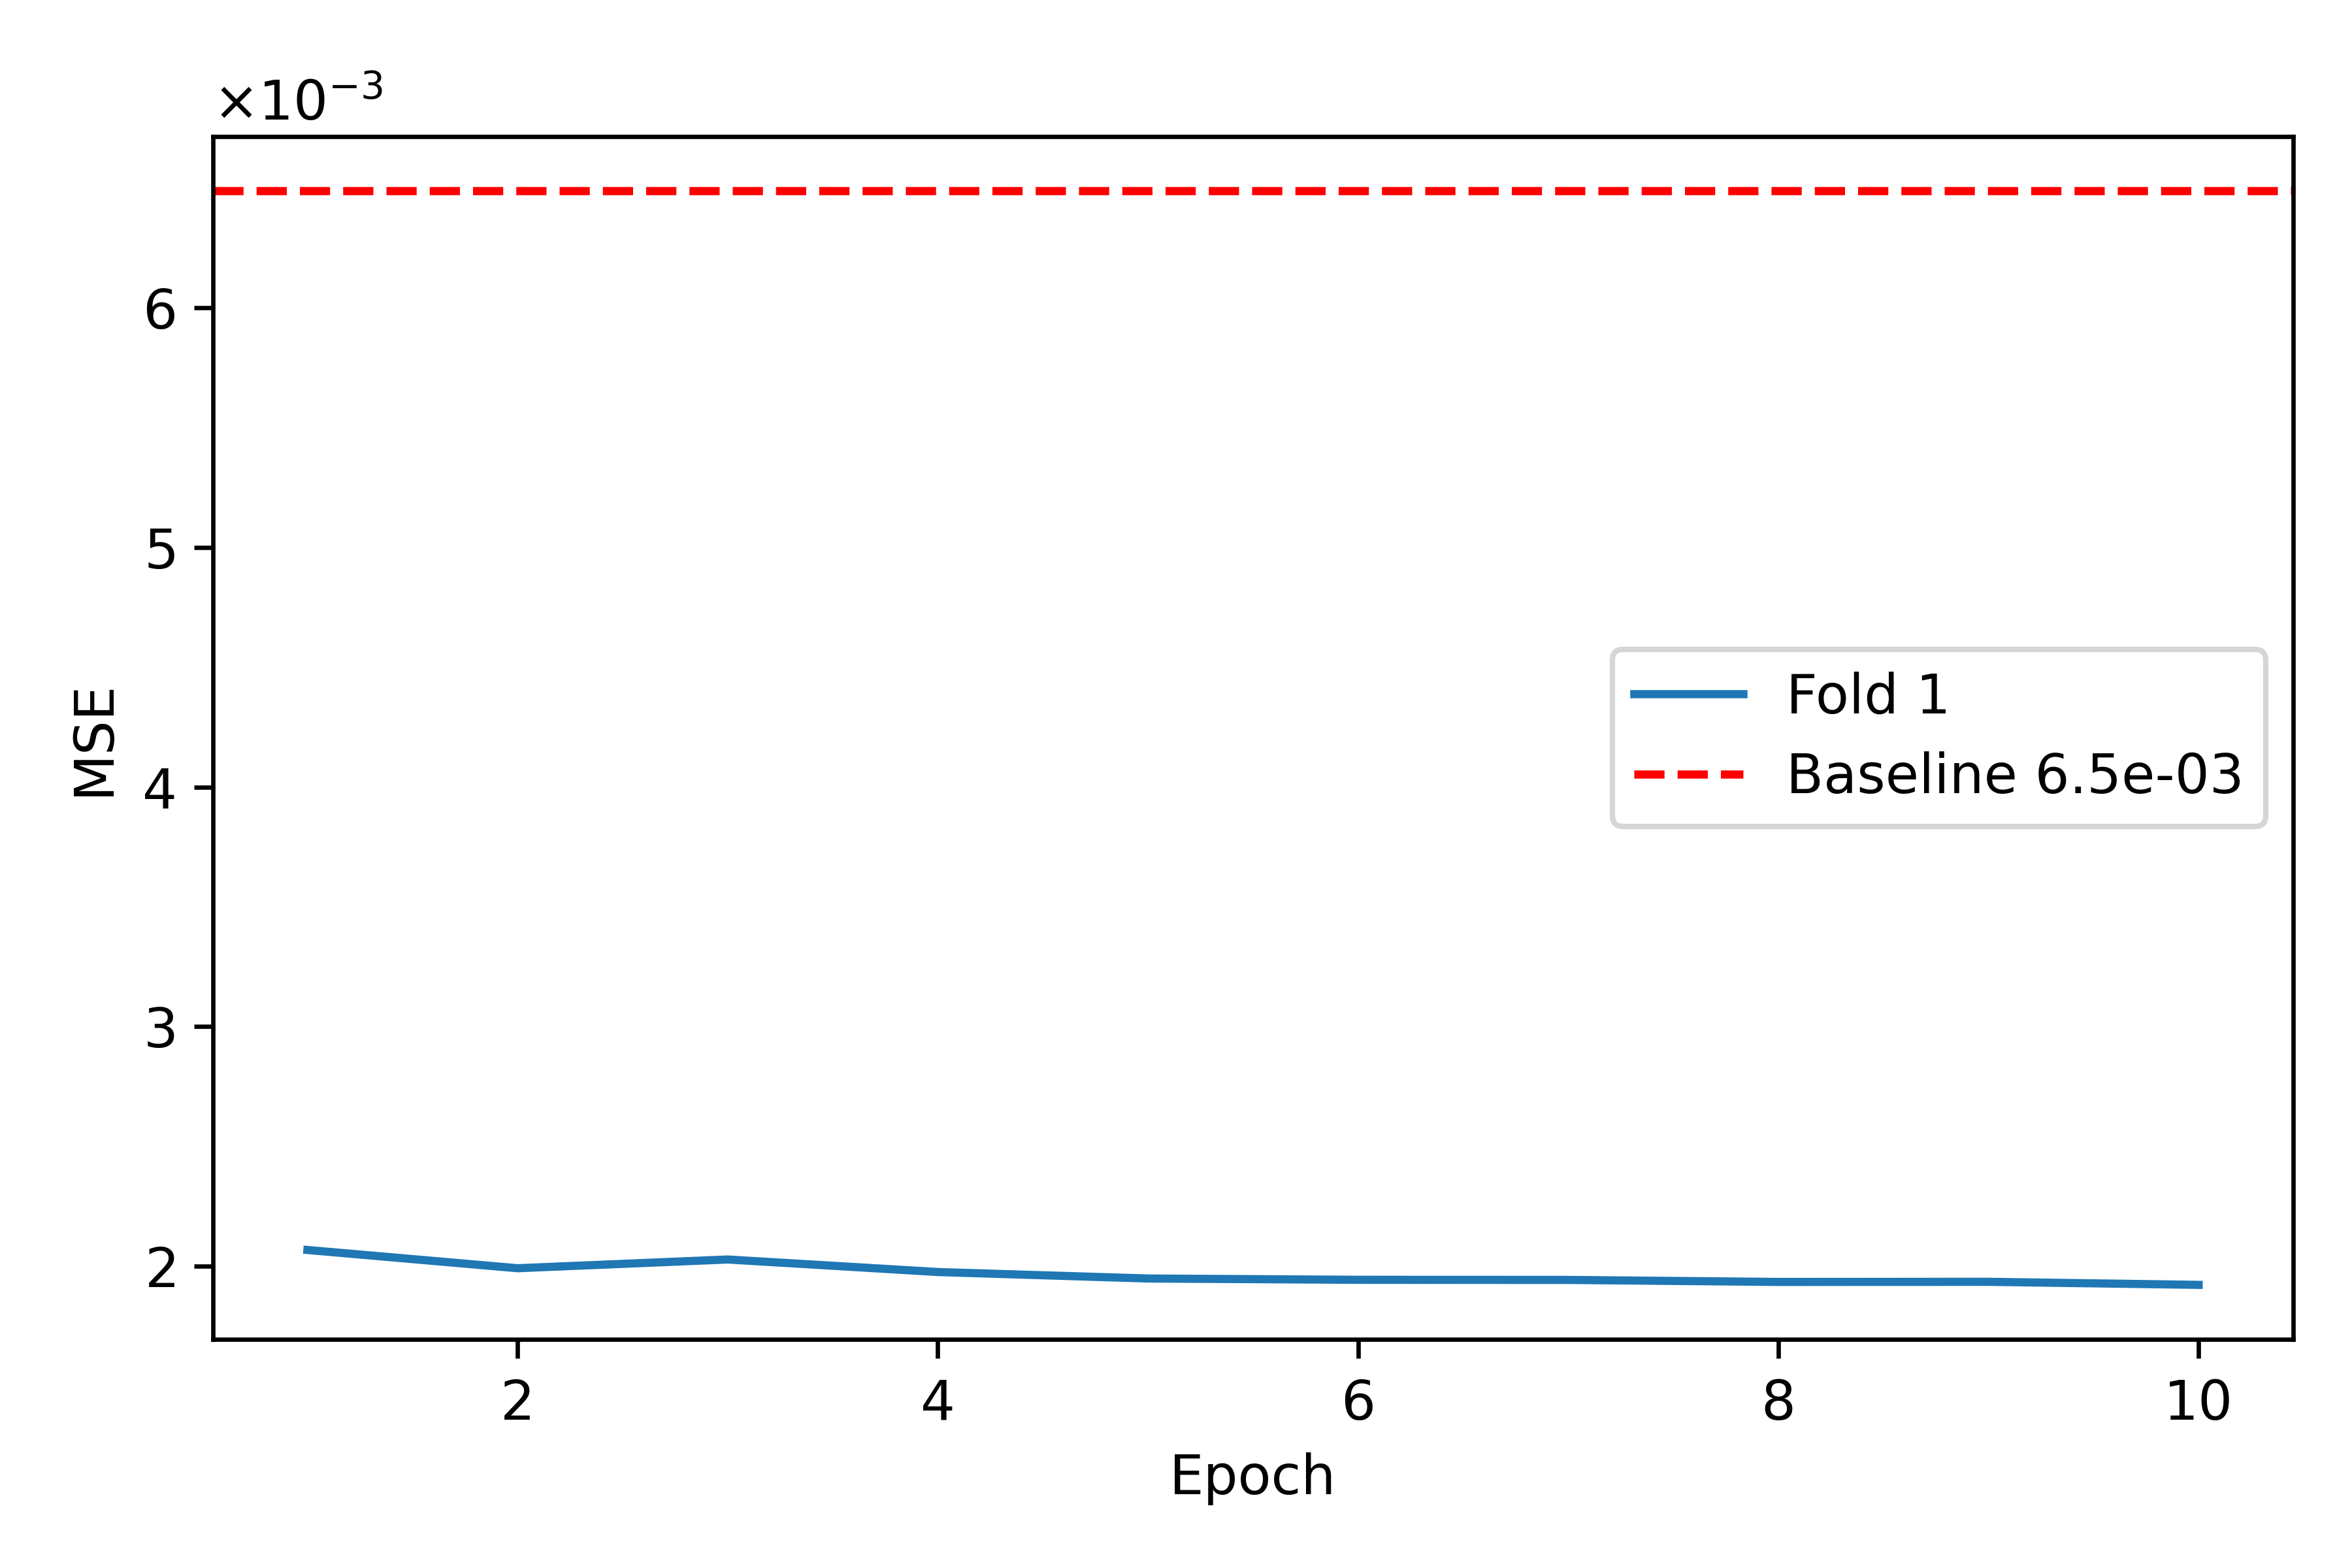
\includegraphics[width=0.8\linewidth]{Plot_MSE_ResUNet.png}
            \vspace{0.1cm} \\
            \small \textbf{ResUNet MSE} \\
        \end{column}
        \begin{column}{0.48\textwidth}
            \centering
            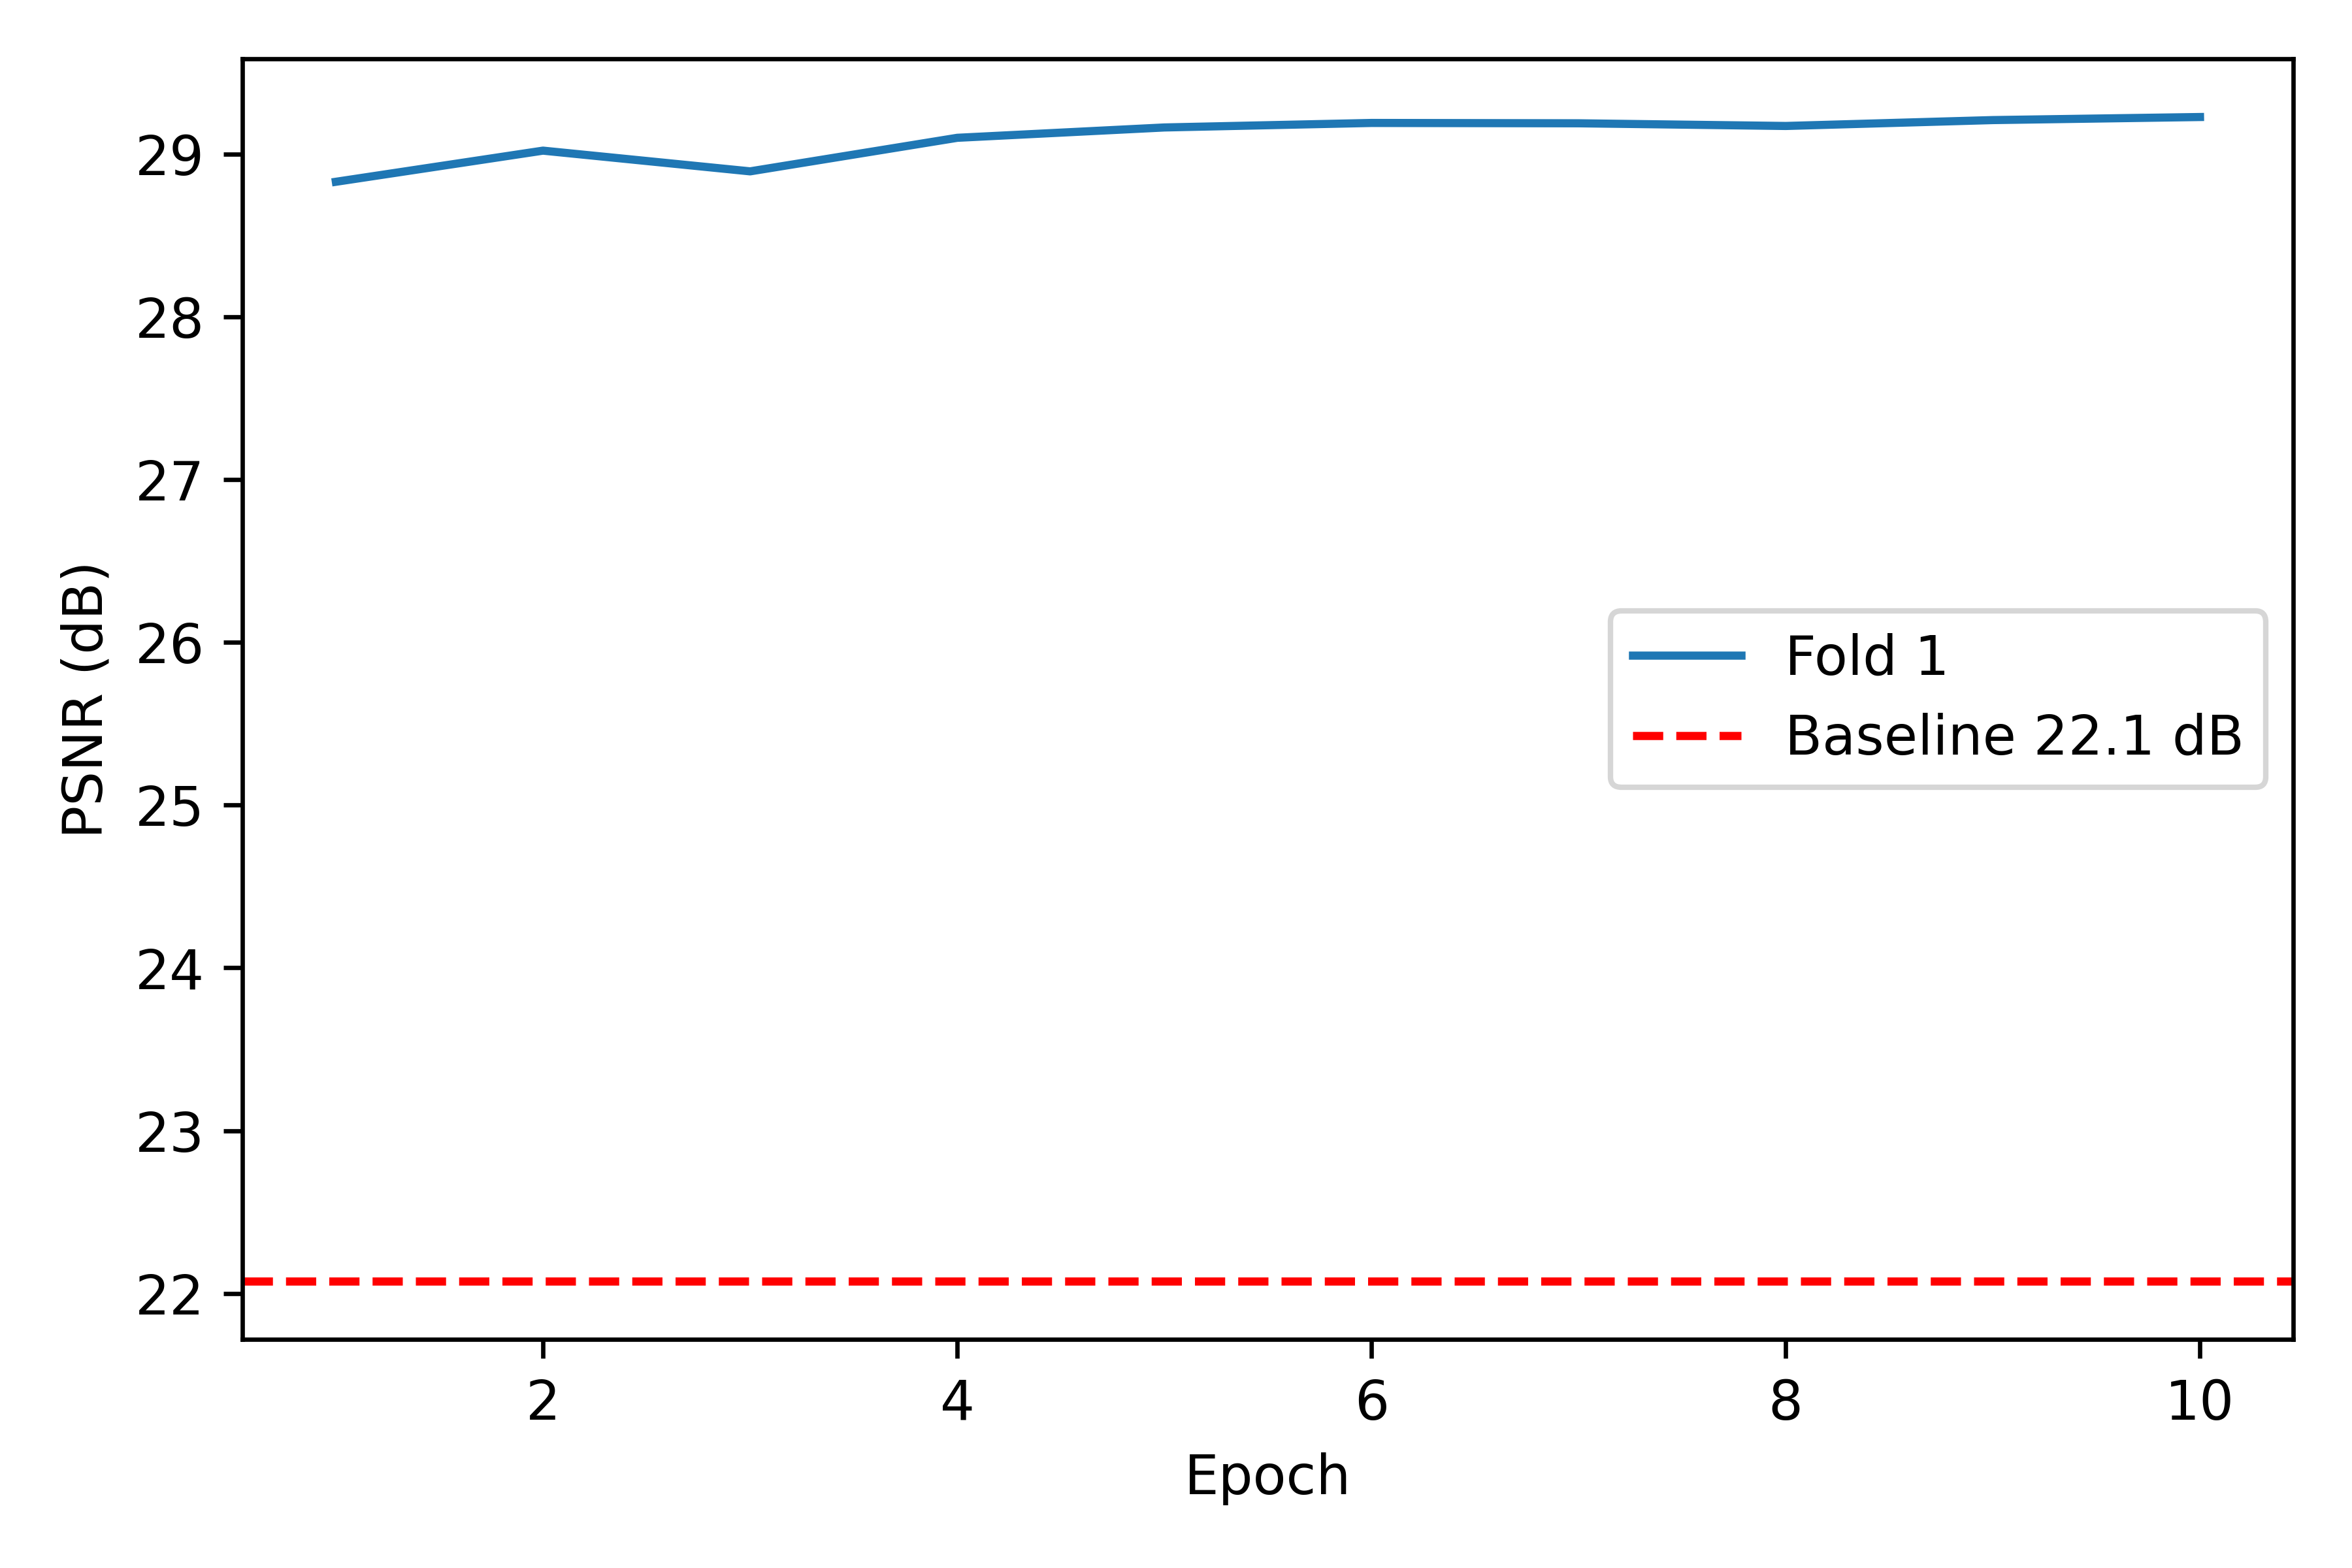
\includegraphics[width=0.8\linewidth]{Plot_PSNR_ResUNet.png}
            \vspace{0.1cm} \\
            \small \textbf{ResUNet PSNR} \\
        \end{column}
    \end{columns}

    \vspace{0.3cm}
    
    % Rândul 2 (Jos)
    \begin{columns}[T]
        \begin{column}{0.48\textwidth}
            \centering
            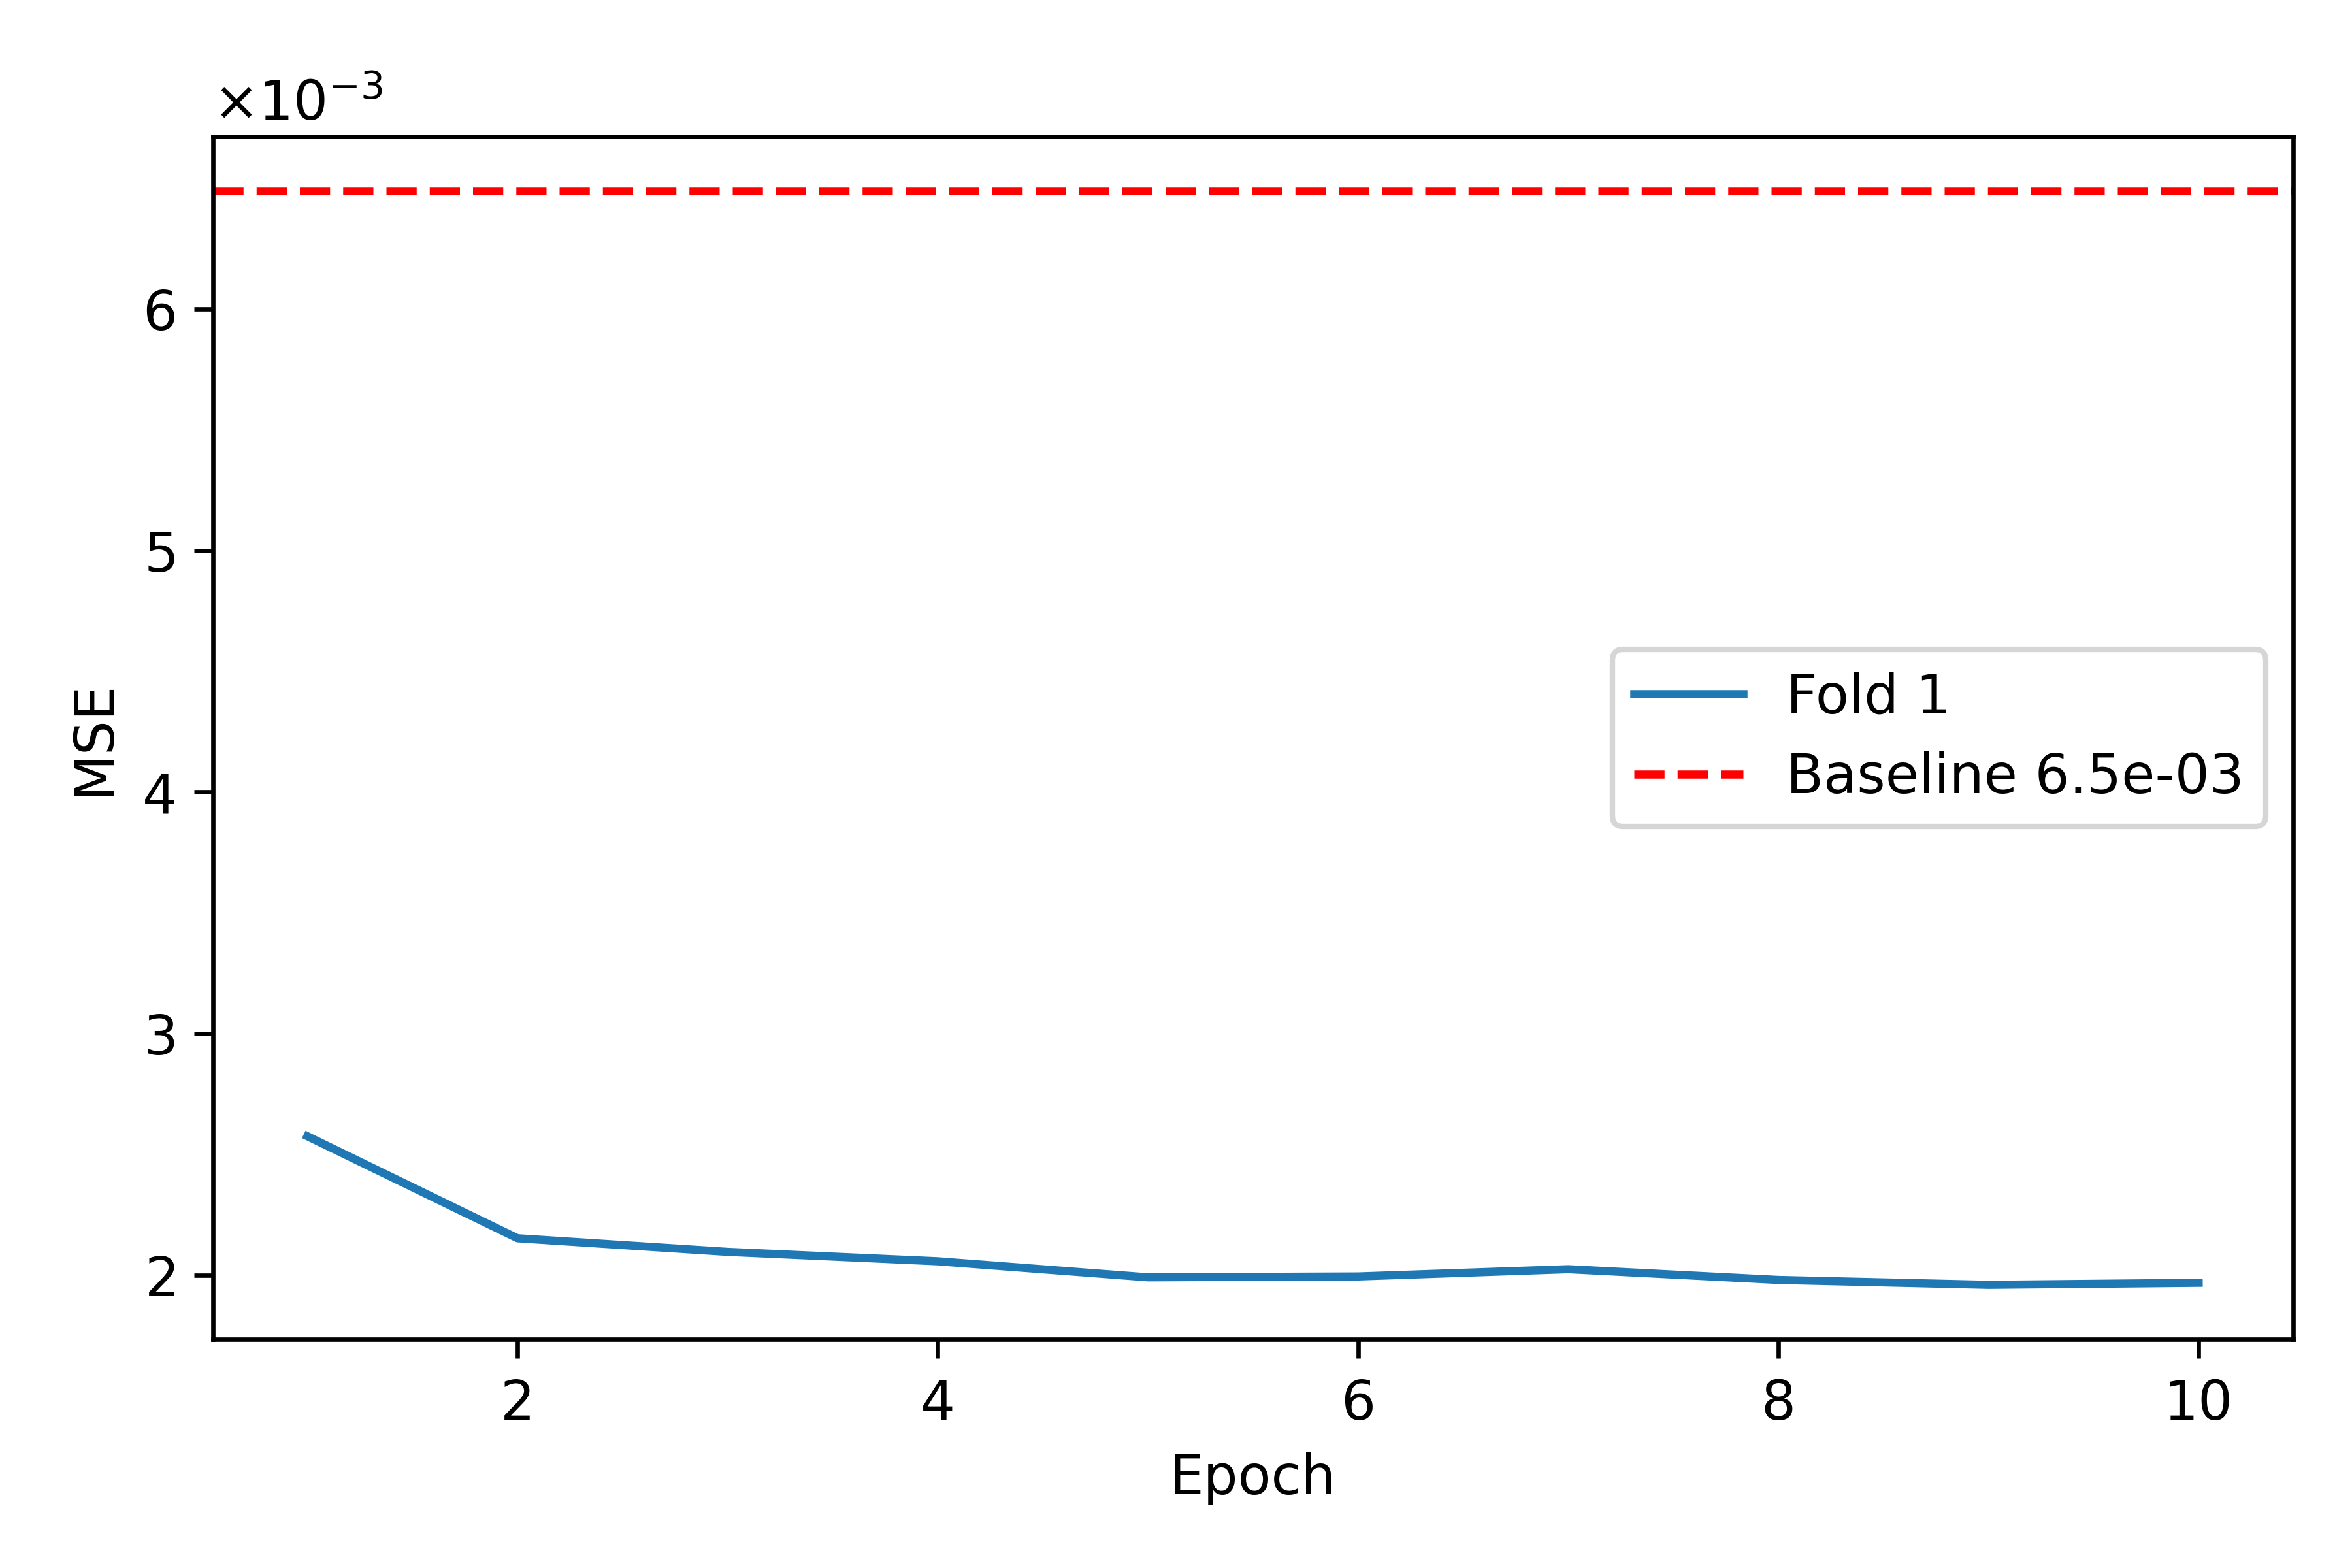
\includegraphics[width=0.8\linewidth]{Plot_MSE_DnCNN.png}
            \vspace{0.1cm} \\
            \small \textbf{DnCNN MSE} \\
        \end{column}
        \begin{column}{0.48\textwidth}
            \centering
            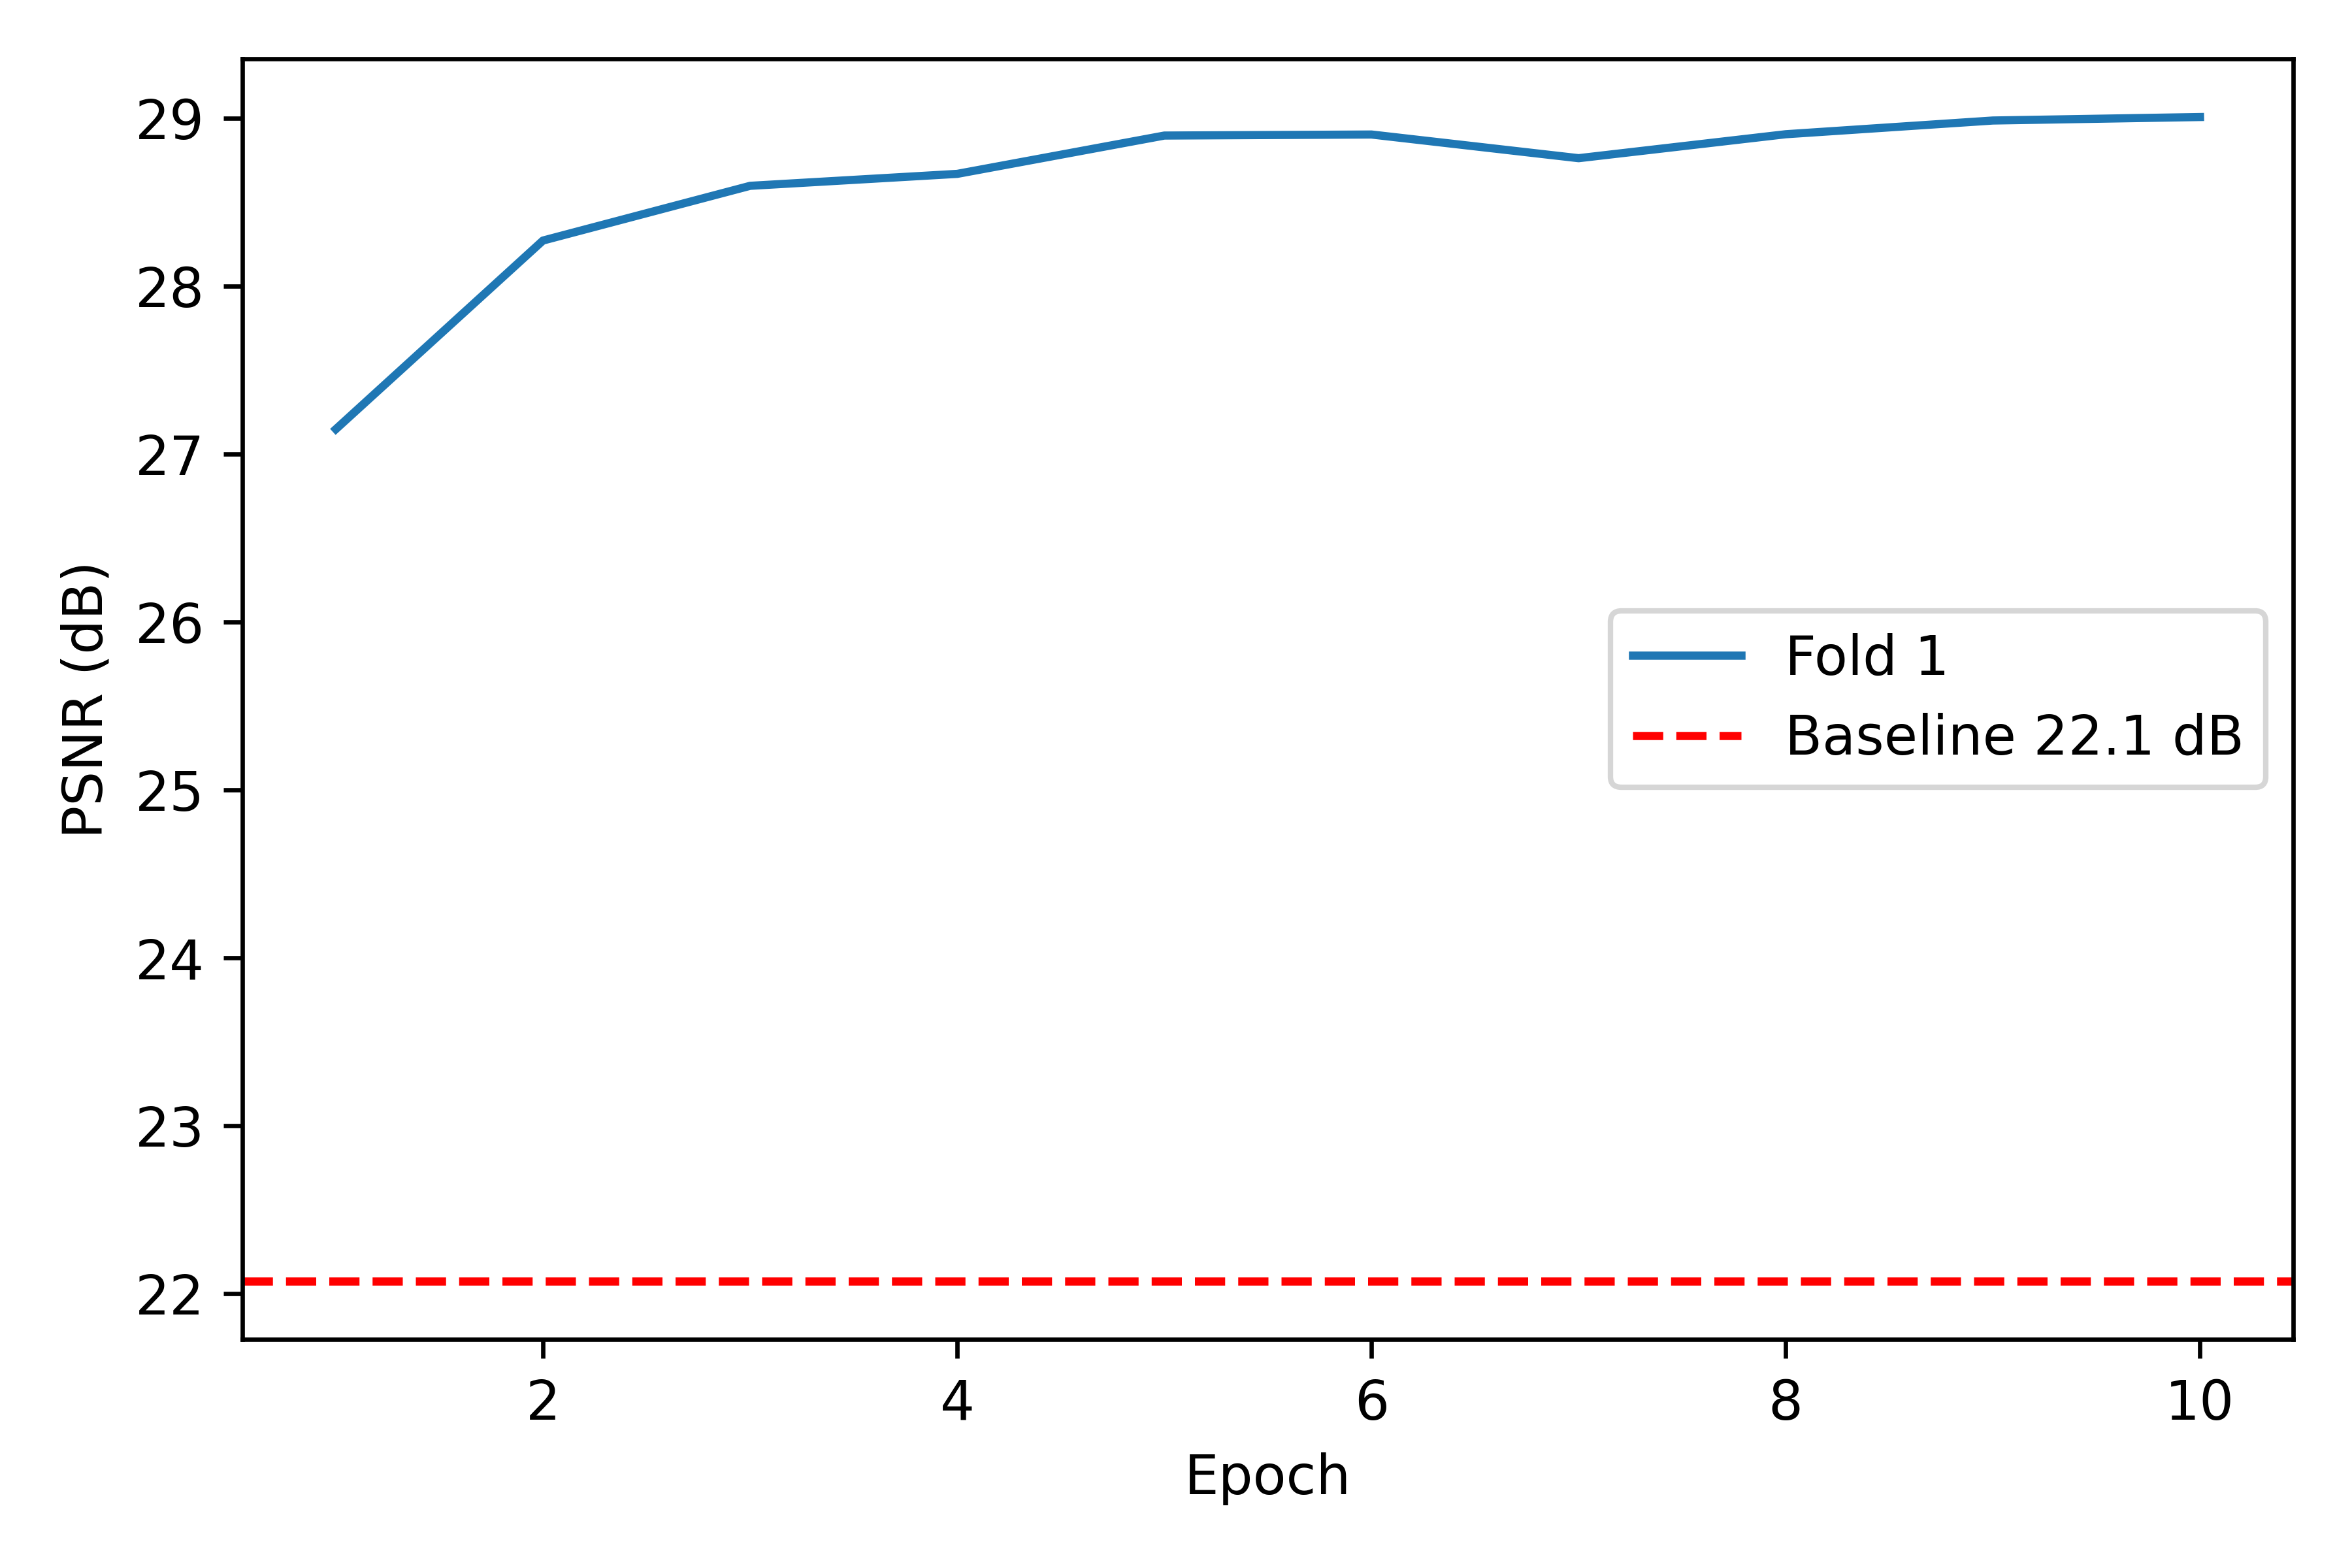
\includegraphics[width=0.8\linewidth]{Plot_PSNR_DnCNN.png}
            \vspace{0.1cm} \\
            \small \textbf{DnCNN PSNR} \\
        \end{column}
    \end{columns}
\end{frame}

\begin{frame}[plain]
    \makebox[\linewidth]{%
        \includegraphics[width=\paperwidth, height=\paperheight, keepaspectratio]{duck_ResUNet_Full.png}%
    }
\end{frame}

\begin{frame}{Performance Across Degradation Profiles}
    \vspace{0.2cm}
    
    \begin{table}[]
        \centering
        \renewcommand{\arraystretch}{1.3}
        \resizebox{\textwidth}{!}{%
        \begin{tabular}{lccccc}
            \toprule
            \textbf{Dataset Profile} & \textbf{Blur ($\sigma$)} & \textbf{Noise ($\sigma$)} & \textbf{PSNR (dB) $\uparrow$} & \textbf{MSE $\downarrow$} \\
            \midrule
            Dataset 1            & 5         & 0                        & 32.90 & 0.0008 \\
            Dataset 2            & 10        & 0                        & 32.76 & 0.0008 \\ 
            Dataset 3            & 15        & 0                        & 32.66 & 0.0008 \\
            Dataset 4            & 0         & 15                       & 29.44 & 0.0011 \\
            Dataset 5            & 0         & 20                       & 28.11 & 0.0018 \\
            Dataset 6            & 0         & 25                       & 26.60 & 0.0024 \\
            Dataset 7            & 10        & 15                       & 24.72 & 0.0037 \\
            \bottomrule
        \end{tabular}%
        }
    \end{table}
    \textbf{Setup:} DnCNN with MSE Loss and 17 layers, trained with k-fold on a subset of 100 images
\end{frame}


%===================================================================================================
% Conclusions
%===================================================================================================
\section{Conclusions}

\begin{frame}{Conclusions \& Future Work}
    \vspace{0.2cm}
    \textbf{Project Outcomes:}
    \begin{itemize}
        \item \textbf{Deep Learning Efficacy:} Convolutional architectures (ResUNet, DnCNN) demonstrate robust capability in simultaneously handling denoising and deblurring, effectively separating noise from critical structural details.
        \item \textbf{Loss Optimization:} Pure MSE optimizes pixel intensity but degrades perceptual quality. Hybrid functions (MAE + SSIM) are essential to prevent over-smoothing and preserve structural integrity.
        \item \textbf{SOTA Benchmarking:} Vision Transformers establish a high performance upper bound, proving highly capable of recovering images from severe, global degradations.
    \end{itemize}

    \vspace{0.4cm}
    \textbf{Future Directions:}
    \begin{itemize}
        \item Evaluate inference time vs. restoration quality trade-offs for potential real-time applications.
        \item Test model robustness on real-world degradation data.
    \end{itemize}
\end{frame}

\begin{frame}{}
    \centering
  
    \vspace{30pt}
    {\LARGE Thank You!}
    
    
    \vspace{20pt}
    \small Team: Vlad-Ștefan Moreanu, Cosmin Eusebiu Pătrașcu \\ Iunie 2026
\end{frame}

\end{document}